Ολοκληρώνοντας τον κύκλο των δοκιμών για τους αλγορίθμους επιβλεπόμενης μάθησης, δημιουργήθηκε η ανάγκη για περαιτέρω έρευνα σε διαφορετικούς αλγορίθμους. Οι αλγόριθμοι επιβλεπόμενης μάθησης έχουν ένα βασικό μειονέκτημα, όταν προσεγγίζεται ένα πραγματικό πρόβλημα. Αυτό είναι η δυσκολίας εφαρμογής του αλγορίθμου, λόγω της έλλειψης των τάξεων των δεδομένων που απαιτεί ένα τέτοιο σύστημα για να εκπαιδευτεί. Η δυσκολία αυτή παρακάμπτεται χρησιμοποιώντας μη-επιβλεπόμενους ή ημι-επιβλεπόμενους αλγορίθμους που απαιτούν λίγα ή και κανένα ταξινομημένο παράδειγμα. Σε αυτό το κεφάλαιο θα προσεγγιστεί το πρόβλημα της ταξινόμησης καταναλωτών με νέα συστήματα που θα μπορούν να έχουν άμεσα χρήση στη λύση του πραγματικού προβλήματος, κάνοντας μια ανασκόπηση στις νέες δυσκολίες που προέκυψαν.
\section{Εξαγωγή Χαρακτηριστικών}
Στο παρόν μέρος θα γίνει παρουσίαση και ανάλυση των χαρακτηριστικών που χρησιμοποιήθηκαν στο μερικώς επιβλεπόμενο σύστημα, αλλά και στο μη επιβλεπόμενο σύστημα. Κάθε παράδειγμα μπορεί να περιγραφεί από ένα συνδιασμό τιμών που αναφέρονται επίσης ως μεταβλητές, χαρακτηριστικά, πεδία ή διαστάσεις. Οι τιμές αυτές μπορούν να είναι διαφορετικού τύπου όπως συνεχείς, δυαδικές ή κατηγορίες. Κάθε παράδειγμα μπορεί να αποτελείται μόνο από μια τιμή (μονοπαραγοντικό) ή και από περισσότερες (πολυπαραγοντική). Στην περίπτωση των πολυπαραγοντικών παραδειγμάτων, όλες οι τιμές μπορεί να είναι ίδιου τύπου ή μπορεί να είναι ένας συνδυασμός διαφορετικών τύπων \cite{Anomaly}.\\
Παράλληλα, κάθε παράδειγμα μπορεί να οριστεί βάση ακόμη δύο δομών ως προς τον ορισμό του προβλήματος \cite{Anomaly}.
\begin{enumerate}
\item{\textit{Τιμές Συσχετισμού}} Τέτοιου είδους τιμές χρησιμοποιούνται για να περιγράψουν ένα γενικό πλαίσιο που χαρακτηρίζει ένα παράδειγμα. Στις χρονοσειρές, ο χρόνος είναι μια τιμή που παρέχει μια σχετικότητα, η οποία καθορίζει τη θέση ενός παραδείγματος σε μια ολόκληρη ακολουθία. Μία τιμή γενικού πλαισίου είναι η μηνιαία κατανάλωση ενός κατοίκου.
\item{\textit{Συμπεριφορικές Τιμές}} Είναι οι τιμές που δεν προδίδουν ένα γενικό πλαίσιο για κάποιο παράδειγμα ή κάποια σχετικότητα. Ένα τέτοιο παράδειγμα θα μπορούσε να είναι η ετήσια παραγωγή ενέργειας σε όλο τον κόσμο.
\end{enumerate}
\subsection{Φύση Χαρακτηριστικών}
Το μερικώς επιβλεπόμενο και μη επιβλεπόμενο σύστημα απαιτούν εισόδους που να δίνουν τη δυνατότητα να διαχωρίζονται σε δύο κλάσεις οι καταναλωτές. Για να γίνει αυτό απαιτείται η χρήση χαρακτηριστικών που να αντιπροσωπεύουν την κλάση, αλλά και χαρακτηριστικά που προσδίνουν γενικότητα στο κάθε παράδειγμα. Με αυτό τον τρόπο παρέχεται ένα περιθώριο στον αλγόριθμο, έτσι ώστε να μπορεί εύκολα να προσαρμόζεται σε καινούργια και ξεχωριστά παραδείγματα. Ένας απλοϊκός τρόπος να διαχωρίσουμε τα χαρακτηριστικά είναι σε χαρακτηριστικά γενίκευσης και σε χαρακτηριστικά διαχωρισμού κλάσεων. Όλα τα παρακάτω χαρακτηριστικά αποτελούν τιμές συσχέτισης.
\subsubsection{Χαρακτηριστικά Γενίκευσης} 
Τα πλεονέκτημα των χαρακτηριστικών γενίκευσης είναι ότι βοηθούν στην κατάταξη του καταναλωτή σε σχέση με τους υπόλοιπους, ώστε να εξαχθούν πληροφορίες, όπως ο τύπος καταναλωτή (οικιακού ή βιομηχανικού) και το προφίλ κατανάλωσής του. Τέτοια χαρακτηριστικά πρέπει να περιορίζονται σε αριθμό όμως, καθώς ενδέχεται να δυσκολεύσουν τον διαχωρισμό με βάση το κριτήριο που θέτουμε παρέχοντας μεγάλο παράγοντα γενίκευσης.  Τέτοιου είδους χαρακτηριστικά είναι τα παρακάτω:
\begin{enumerate}
\item{\textit{Ετήσια μέση τιμή ημίωρου}} Βρίσκεται ο μέσος όρος ημίωρου κάθε μέρας και για όλες τις μέρες του έτους βρίσκεται ο ετήσιος μέσος όρος.
\item{\textit{Ετήσια τυπική απόκλιση ημίωρου}} Βρίσκεται η τυπική απόκλιση κάθε μέρας και για όλες τις μέρες του έτους βρίσκεται ο ετήσιος μέσος όρος της τυπικής απόκλισης.
\item{\textit{Διαφορά Ετήσιου Ελάχιστου τάσης με όμοιους}} Βάση αυτού του χαρακηριστικού ορίζεται για όμοιους καταναλωτές το ελάχιστο της τάσης κατανάλωσής τους και στην συνέχεια βρίσκεται η απόλυτη διαφορά σε  ημέρες.
\item{\textit{Διαφορά μέσης τιμής με ομοίους}} Με αυτό το χαρακτηριστικό βρίσκεται η διαφορά του ετήσιου μέσου όρου κάθε καταναλωτή με την ομάδα καταναλωτών που ανήκει.
\item{\textit{Διαφορά τυπικής απόκλισης με ομοίους}} Με αυτό το χαρακτηριστικό βρίσκεται η διαφορά της ετήσιας τυπικής απόκλισης κάθε καταναλωτή με την ομάδα καταναλωτών που ανήκει.
\end{enumerate}
\subsubsection{Χαρακτηριστικά Διαχωρισμού}
Τα χαρακτηριστικά διαχωρισμού επικεντρώνονται στην όξυνση των διαφορών μεταξύ των καταναλωτών διαφορετικών κλάσεων. Λειτουργούν, λοιπόν σαν οδηγοί για τον αλγόριθμο ώστε να κάνουν πιο εμφανείς τις διαφορές των κλάσεων. Το πλεονέκτημα τους είναι ο παράγοντας εξειδίκευσης που παρέχουν στον αλγόριθμο διευκολύνοντας τον να αναγνωρίζει με διαφορετικούς τρόπους κάθε κλάση. Το μειονέκτημα είναι πως λόγο της εξειδικευμένης τους φύσης μπορεί να μην εφαρμόζονται απόλυτα από όλους τους καταναλωτές ή στην χειρότερη περίπτωση να περιγράφουν μια σπάνια συμπεριφορά που δεν ενδιαφερόμαστε να διαχωρίσουμε.
\begin{enumerate}
\item{\textit{Κινούμενος μέσος όρος μηνιαίου μέσου όρου}} Πρόκειται για υπό συνθήκη χαρακτηριστικό που αν παρατηρήσει κάποια σημαντική πτώση των καταναλώσεων τότε ψάχνει για την μέγιστη και την καταγράφει. Ορίζοντας ως $min$ τον μήνα του ελαχίστου και $c$ την κατανάλωση του αντίστοιχου $i$ μήνα θα έχω την εξής φόρμουλα για αυτό το χαρακτηριστικό. 
\begin{center}
\resizebox{8cm}{!}{$\bar{c_{p}}-\bar{c_{a}}=\frac{1}{k-1}\sum_{i=1}^{k} c_{m-i}-\frac{1}{w}\sum_{i=0}^{w}  c_{m+i}$}
\end{center}
\item{\textit{Κινούμενος μέσος όρος μηνιαίας τυπικής απόκλισης}} Πρόκειται για υπό συνθήκη χαρακτηριστικό που αν παρατηρήσει κάποια σημαντική πτώση της τυπικής απόκλισης τότε ψάχνει για την μέγιστη και την καταγράφει. Ορίζοντας ως $min$ τον μήνα του ελαχίστου και $std$ την τυπική απόκλιση της κατανάλωσης τον αντίστοιχο $i$ μήνα θα έχω την εξής φόρμουλα για αυτό το χαρακτηριστικό. 
\begin{center}
\resizebox{8.8cm}{!}{$\bar{std_{p}}-\bar{std_{a}}=\frac{1}{k-1}\sum_{i=1}^{k} std_{m-i}-\frac{1}{w}\sum_{i=0}^{w}  std_{m+i}$}
\end{center}
\item{\textit{Συμμετρική διαφορά καταναλώσεων}} Πρόκειται για υπό συνθήκη χαρακτηριστικό που παρατηρεί μια γενική συμπεριφορά όμοιων καταναλωτών ως προς τη χρονική στιγμή της ελάχιστης κατανάλωσης και ψάχνει για κάποια σημαντική πτώση της κατανάλωσης ανάμεσα σε 2 συμμετρικές χρονικές στιγμές με άξονα συμμετρίας την εκάστοτε χρονική στιγμή ελαχίστου. Ορίζοντας ως $min$ την ημέρα του ελαχίστου και $c$ την κατανάλωση της αντίστοιχης $i$ ημέρα θα έχω τις εξής φόρμουλες εισάγοντας σε αυτό το σημείο και την ευκλείδεια απόσταση.
\begin{center}
\resizebox{8cm}{!}{$\bar{c_{p}}-\bar{c_{a}}=\frac{1}{n}\sum_{i=1}^{n+1} c_{min-i}-\frac{1}{n}\sum_{i=0}^{n}  c_{min+i}$}
\resizebox{9cm}{!}{$||c_{p}||-||c_{a}||=\sqrt{\sum_{i=1}^{n+1} (c_{min-i})^2}-\sqrt{\sum_{i=0}^{n}  (c_{min+i})^2}$}
\end{center}
\item{\textit{Συμμετρική διαφορά τυπικής απόκλισης}} Πρόκειται για υπό συνθήκη χαρακτηριστικό που παρατηρεί μια γενική συμπεριφορά όμοιων καταναλωτών ως προς τη χρονική στιγμή της ελάχιστης κατανάλωσης και ψάχνει για κάποια σημαντική πτώση της τυπικής απόκλισης ανάμεσα σε 2 συμμετρικές χρονικές στιγμές με άξονα συμμετρίας την εκάστοτε χρονική στιγμή ελαχίστου. Ορίζοντας ως $min$ την ημέρα του ελαχίστου και $std$ την την τυπική απόκλιση της κατανάλωσης την αντίστοιχη $i$ ημέρα θα έχω τις εξής φόρμουλα για αυτό το χαρακτηριστικό. 
\begin{center}
\resizebox{9cm}{!}{$\bar{std_{p}}-\bar{std_{a}}=\frac{1}{n}\sum_{i=1}^{n+1} std_{min-i}-\frac{1}{n}\sum_{i=0}^{n}  std_{min+i}$}
\resizebox{10cm}{!}{$||std_{p}||-||std_{a}||=\sqrt{\sum_{i=1}^{n+1} (std_{min-i})^2}-\sqrt{\sum_{i=0}^{n}  (std_{min+i})^2}$}
\end{center}
\item{\textit{Τμηματική διαφορά κατανάλωσης με όμοιους καταναλωτές}} Πρόκειται για υπό συνθήκη χαρακτηριστικό που παρατηρεί μια γενική συμπεριφορά όμοιων καταναλωτών ως προς τη χρονική στιγμή της ελάχιστης κατανάλωσης και ψάχνει για κάποια σημαντική πτώση της κατανάλωσης ανάμεσα στον καταναλωτή και τους όμοιούς του μετά την χρονική στιγμή της ελάχιστης κατανάλωσης. Πιο φορμαλιστικά θεωρώντας τους όρους $c_{cl}$ την τυπική κατανάλωση μιας ομάδας και $c_{co}$ την κατανάλωση ενός καταναλωτή έχουμε την παρακάτω διαφορά μέσων όρων και νορμών των καταναλώσεων.
\begin{center}
\resizebox{9cm}{!}{$\bar{c_{cl}}-\bar{c_{co}}=\frac{1}{n}\sum_{i=1}^{n+1} c_{cl,min-i}-\frac{1}{n}\sum_{i=0}^{n}  c_{co,min+i}$}
\resizebox{10cm}{!}{$||c_{cl}||-||c_{co}||=\sqrt{\sum_{i=1}^{n+1} (c_{cl,min-i})^2}-\sqrt{\sum_{i=0}^{n}  (c_{co,min+i})^2}$}
\end{center}
\item{\textit{Τμηματική διαφορά τυπικής απόκλισης με όμοιους καταναλωτές}} Πρόκειται για υπό συνθήκη χαρακτηριστικό που παρατηρεί μια γενική συμπεριφορά όμοιων καταναλωτών ως προς τη χρονική στιγμή της ελάχιστης κατανάλωσης και ψάχνει για κάποια σημαντική πτώση της τυπικής απόκλισης ανάμεσα στον καταναλωτή και τους όμοιούς του μετά την χρονική στιγμή της ελάχιστης κατανάλωσης. Πιο φορμαλιστικά θεωρώντας τους όρους $std_{cl}$ την τυπική κατανάλωση μιας ομάδας και $std_{co}$ την κατανάλωση ενός καταναλωτή έχουμε την παρακάτω διαφορά μέσων όρων και νορμών των τυπικών αποκλίσεων των καταναλώσεων.
\begin{center}
\resizebox{10cm}{!}{$\bar{std_{cl}}-\bar{std_{co}}=\frac{1}{n}\sum_{i=0}^{n}  std_{cl,min+i}-\frac{1}{n}\sum_{i=0}^{n}  std_{co,min+i}$}
\resizebox{11cm}{!}{$||std_{cl}||-||std_{co}||=\sqrt{\sum_{i=0}^{n} (std_{cl,min+i})^2}-\sqrt{\sum_{i=0}^{n}  (std_{co,min+i})^2}$}
\end{center}
\item{\textit{Χρονική Διαφορά Ελαχίστου}} Πρόκειται για υπό συνθήκη χαρακτηριστικό που εξερευνά το ελάχιστο χρονικό σημείο της τάσης της καμπύλης κάθε καταναλωτή. Με βάση την ομάδα που ανήκει κάθε καταναλωτής υπολογίζεται η απόλυτη τιμή της χρονικής διαφοράς μεταξύ του ελαχίστου κάθε καταναλωτή με την ομάδα που ανήκει. Χρησιμοποιώντας ένα όριο για τη διαφορά αυτή γίνεται αντιληπτή οποιαδήποτε έντονη διακύμανση του καταναλωτή με την ομάδα του και καταγράφεται σαν χαρακτηριστικό διαχωρισμού από την αναμενόμενη συμπεριφορά κατανάλωσης.
\begin{center}
\resizebox{3.5cm}{!}{$|t_{cl,min}-t_{co,min}|$}
\end{center}
\end{enumerate}

\subsection{Δοκιμή Χαρακτηριστικών με σταθερή απάτη}
Αφού οριστούν τα χαρακτηριστικά που εκτιμάται ότι μπορούν να βοηθήσουν στον διαχωρισμό των κλάσεων, έπεται φυσικά η δοκιμή τους με έναν αφελή τρόπο, έτσι ώστε να επιβεβαιωθεί ότι μπορούν να λειτουργήσουν όπως αναμένεται. Παράλληλα, η δοκιμή αυτή παρέχει μεγάλο όγκο πληροφορίας, αφού καθιστά εμφανή τα σημεία και τις προϋποθέσεις που τα χαρακτηριστικά έχουν μεγάλη ακρίβεια, αλλά και εκεί που υστερούν.

Ο κώδικας της δοκιμής θεωρεί δεδομένη και σταθερή την ένταση κλοπής και την ημέρα που κάθε καταναλωτής ξεκινά να αλλοιώνει τις τιμές του. Ειδικότερα, το ποσοστό των καταναλωτών που αλλοιώνει τις μετρήσεις του είναι 50 τοις εκατό, η ένταση της κλοπής είναι της τάξης του 80 τοις εκατό και η μέρα κλοπής ορίζεται η 182η, δηλαδή μετά από 6 μήνες κανονικής κατανάλωσης ο χρήστης εισάγει σύστημα αλλοίωσης της μέτρησής του. Δοκιμάζοντας ξεχωριστά τα χαρακτηριστικά διαχωρισμού ελέγχουμε το όριο κάθε χαρακτηριστικού έτσι ώστε να δώσει μεγαλύτερη ακρίβεια στις επιθέσεις δεδομένων υπό τις παραπάνω συνθήκες. Αν ο παρατηρηθούν τέτοια χαρακτηριστικά ο καταναλωτής θεωρείται θετικός στην κλοπή. Αντίθετα αν ο καταναλωτής δεν έχει την αναμενόμενη συμπεριφορά το χαρακτηριστικό δεν καταγράφει κάποια τιμή και ο καταναλωτής θεωρείται αρνητικός στην κλοπή. Αναλυτικότερα για κάθε χαρακτηριστικό διαχωρισμού λήφθηκαν τα παρακάτω αποτελέσματα:
\begin{enumerate}
\item{\textit{Κινούμενος μέσος όρος μηνιαίου μέσου όρου}} \\
Στην πρώτη δοκιμή δόθηκε έμφαση στη γενικότερη συμπεριφορά του χαρακτηριστικού ως προς το όριο που τίθεται κάθε φορά. Έτσι παρατηρείται εύκολα πως για μεγάλο όριο ο διαχωρισμός έχει χαμηλή ακρίβεια με εξαιρετικά μικρό ποσοστό αποτυχίας. Αντίθετα, αν το όριο χαμηλώσει αισθητά ο χάνεται η έννοια του διαχωρισμού και ο αλγόριθμος θεωρεί θετικούς σε κλοπές σχεδόν όλους τους καταναλωτές.
\begin{center}
\begin{longtabu}  to 0.8\textwidth { | X[c] || X[c] | X[c] | X[c] | X[c] | X[c] |  }
 \hline
  Όριο & \en{DR}  & \en{FPR} & \en{BDR} & \en{Accuracy} & \en{F1}\\
 \hline
 0,8&	44,8&	1,4	&0,97	&71,7&	61,29\\
0,7&	98,7&	1,9	&0,98	&98,4&	98,4\\
0,6&	99,3&	3,6&	0,97&	97,85&	97,88\\
0,5&	99,8&	7,5	&0,93	&96,15&	96,15\\
0&	99,9&	91,5	&0,52	&54,2&	68,57\\
\hline
\caption{Δοκιμή 1ου χαρακτηριστικού}
\label{testfeat1}
\end{longtabu}
\end{center}

\item{\textit{Κινούμενος μέσος όρος μηνιαίας τυπικής απόκλισης}} \\
Αντίστοιχα και εδώ για παρόμοιες τιμές του ορίου με το προηγούμενο χαρακτηριστικό ο διαχωρισμός είναι εξαιρετικά εύστοχος και δεν αφήνει περιθώρια για αμφισβήτηση.
\begin{center}
\begin{longtabu} to 0.8\textwidth { | X[c] || X[c] | X[c] | X[c] | X[c] | X[c] |  }
 \hline
  Όριο & \en{DR}  & \en{FPR} & \en{BDR} & \en{Accuracy} & \en{F1}\\
 \hline
0,7	&98,2	&2,3	&0,98	&98,3	&98,31\\
0,6	&99,8	&4,1	&0,96	&97,85	&97,89\\
0,5	&99,5	&8,2	&0,92	&95,65	&95,81\\
\hline
\caption{Δοκιμή 2ου χαρακτηριστικού}
\label{testfeat2}
\end{longtabu}
\end{center}
\item{\textit{Συμμετρική διαφορά καταναλώσεων}} \\
Το συγκεκριμένο χαρακτηριστικό δεν δίνει αξιόπιστα αποτελέσματα, καθώς η συμμετρία που προκύπτει από τον χρησιμοποιούμενο τύπο απάτης κάνει το συγκεκριμένο χαρακτηριστικό να αποτυγχάνει σε αυτή τη δοκιμή. Παρόλα αυτά, το χαμηλό ποσοστό αποτυχίας αφήνει δεύτερες σκέψεις, καθώς δεν επιβαρύνει αισθητά τα αποτελέσματα, αλλά βοηθά στη γενίκευση του τύπου κλοπής. 
\begin{center}
\begin{longtabu} to 0.8\textwidth { | X[c] || X[c] | X[c] | X[c] | X[c] | X[c] |  }
 \hline
  Όριο & \en{DR}  & \en{FPR} & \en{BDR} & \en{Accuracy} & \en{F1}\\
 \hline
 0,1&	26,3&	5,7&	0,82&	60,3&	39,85\\
\hline
\caption{Δοκιμή 3ου χαρακτηριστικού}
\label{testfeat3}
\end{longtabu}
\end{center}
Η δοκιμή συνεχίστηκε και με τις νόρμες των καταναλώσεων, παρατηρώντας ελάχιστη βελτίωση στο \en{DR}, ενώ αισθητά καλύτερα αποτελέσματα παρατηρούνται στο \en{FPR} που μειώθηκε ακόμη περισσότερο.
\begin{center}
\begin{longtabu} to 0.8\textwidth { | X[c] || X[c] | X[c] | X[c] | X[c] | X[c] |  }
 \hline
  Όριο & \en{DR}  & \en{FPR} & \en{BDR} & \en{Accuracy} & \en{F1}\\
 \hline
 0,3&	29&	2,1&	0,93&	63,65&	44,71\\
\hline
\caption{Δοκιμή 3ου χαρακτηριστικού με νόρμες}
\label{testfeat3norms}
\end{longtabu}
\end{center}

\item{\textit{Συμμετρική διαφορά τυπικής απόκλισης}} \\
Αντίστοιχα συμπεράσματα ισχύουν και στη συμμετρική διαφορά τυπικής απόκλισης που οριακά ξεπερνά το 10 τοις εκατό στο \en{FPR}. Η γενίκευση που προσφέρει παρόλα αυτά το συγκεκριμένο χαρακτηριστικό είναι χρήσιμη, καθώς εν τέλει όλα τα χαρακτηριστικά θα ενώσουν τα δυνατά τους σημεία για να διαχωρίσουν απάτες με μεγαλύτερο τυχαίο παράγοντα.
\begin{center}
\begin{longtabu} to 0.8\textwidth { | X[c] || X[c] | X[c] | X[c] | X[c] | X[c] |  }
 \hline
  Όριο & \en{DR}  & \en{FPR} & \en{BDR} & \en{Accuracy} & \en{F1}\\
 \hline
 0,1&	38,9&	10,2&	0,79&	64,35&	52,18 \\
\hline
\caption{Δοκιμή 4ου χαρακτηριστικού}
\label{testfeat4}
\end{longtabu}
\end{center}
Σε αυτό το σημείο η μείωση του \en{FPR} είναι αρκετά σημαντικό ζήτημα που τελικώς επιτεύχθει με τις νόρμες που μπόρεσαν να μειώσουν το \en{FPR} χωρίς να επηρεάσουν αρνητικά το \en{DR}. 
\begin{center}
\begin{longtabu} to 0.8\textwidth { | X[c] || X[c] | X[c] | X[c] | X[c] | X[c] |  }
 \hline
  Όριο & \en{DR}  & \en{FPR} & \en{BDR} & \en{Accuracy} & \en{F1}\\
 \hline
0,1&	40,2&	8,9&	0,82&	65,65&	53,92\\
\hline
\caption{Δοκιμή 4ου χαρακτηριστικού με νόρμες}
\label{testfeat4norms}
\end{longtabu}
\end{center}

\item{\textit{Τμηματική διαφορά κατανάλωσης με όμοιους καταναλωτές}} \\
Σε αυτό το χαρακτηριστικό παρατηρείται σχετική αστοχία σε σχέση με τα πρώτα χαρακτηριστικά υποδεικνύοντας ανάγκη για καλύτερη ρύθμιση του χαρακτηριστικού. 
\begin{center}
\begin{longtabu} to 0.8\textwidth { | X[c] || X[c] | X[c] | X[c] | X[c] | X[c] |  }
 \hline
  Όριο & \en{DR}  & \en{FPR} & \en{BDR} & \en{Accuracy} & \en{F1}\\
 \hline
 0,1&	98,4&	11,4&	0,9&	93,5&	93,8\\
0,2&	93,9&	7&	0,93&	93,45	&93,48\\
0,3&	88,3&	4,9&	0,95&	91,7	&91,41\\
\hline
\caption{Δοκιμή 5ου χαρακτηριστικού}
\label{testfeat5}
\end{longtabu}
\end{center}
Δεδομένης της διαφοράς των καταναλώσεων με την γενικευμένη κατανάλωση μιας ομάδας δημιουργείται η ανάγκη για κανονικοποίηση σε κάθε διάνυσμα κατανάλωσης. Με αυτό τον τρόπο επιτυγχάνονται πολύ καλύτερα αποτελέσματα.
\begin{center}
\begin{longtabu} to 0.8\textwidth { | X[c] || X[c] | X[c] | X[c] | X[c] | X[c] |  }
 \hline
  Όριο & \en{DR}  & \en{FPR} & \en{BDR} & \en{Accuracy} & \en{F1}\\
 \hline
 0,3&	98,9&	5,4&	0,95&	96,75&	96,82\\
\hline
\caption{Δοκιμή 5ου χαρακτηριστικού με κανονικοποίηση}
\label{testfeat5normalized}
\end{longtabu}
\end{center}

\begin{center}
\begin{longtabu} to 0.8\textwidth { | X[c] || X[c] | X[c] | X[c] | X[c] | X[c] |  }
 \hline
  Όριο & \en{DR}  & \en{FPR} & \en{BDR} & \en{Accuracy} & \en{F1}\\
 \hline
0,1&	98,7&	7&	0,93&	95,85&	95,96\\
0,2&	97,6&	4,4&	0,96&	96,6&	96,63\\
\hline
\caption{Δοκιμή 5ου χαρακτηριστικού με κανονικοποίηση και νόρμες}
\label{testfeat5normalizednorms}
\end{longtabu}
\end{center}

\item{\textit{Τμηματική διαφορά τυπικής απόκλισης με όμοιους καταναλωτές}} \\
Αντίστοιχη μεθοδολογία εφαρμόστηκε και σε αυτό το χαρακτηριστικό. Τα αποτελέσματα ήταν ικανοποιητικά, αλλά όχι αρκετά. Έτσι χρησιμοποιήθηκε κανονικοποίηση για μπορέσει να μειωθεί το \en{FPR}, ενώ αυξάνεται το \en{DR}.
\begin{center}
\begin{longtabu} to 0.8\textwidth { | X[c] || X[c] | X[c] | X[c] | X[c] | X[c] |  }
 \hline
  Όριο & \en{DR}  & \en{FPR} & \en{BDR} & \en{Accuracy} & \en{F1}\\
 \hline
 0,1&	99,4&	16,1&	0,86&	91,65&	92,25\\
0,2&	95,7&	8,3&	0,92&	93,7&	93,82\\
0,3&	89,8&	6,2&	0,94&	91,8&	91,63\\
\hline
\caption{Δοκιμή 6ου χαρακτηριστικού}
\label{testfeat6}
\end{longtabu}
\end{center}

\begin{center}
\begin{longtabu} to 0.8\textwidth { | X[c] || X[c] | X[c] | X[c] | X[c] | X[c] |  }
 \hline
  Όριο & \en{DR}  & \en{FPR} & \en{BDR} & \en{Accuracy} & \en{F1}\\
 \hline
 0,4&	97&	4,9&	0,95&	96,05&	96,09\\
0,3	&96,3&	5,3&	0,95&	95,5&	95,54\\
\hline
\caption{Δοκιμή 6ου χαρακτηριστικού με κανονικοποίηση}
\label{testfeat6normalized}
\end{longtabu}
\end{center}

\begin{center}
\begin{longtabu} to 0.8\textwidth { | X[c] || X[c] | X[c] | X[c] | X[c] | X[c] |  }
 \hline
  Όριο & \en{DR}  & \en{FPR} & \en{BDR} & \en{Accuracy} & \en{F1}\\
 \hline
0,2&	98,5&	4,5&	0,96&	97&	97,04\\
0,1&	99,2&	5,3&	0,95&	96,95&	97,02\\
\hline
\caption{Δοκιμή 6ου χαρακτηριστικού με κανονικοποίηση και νόρμες}
\label{testfeat6normalizednorms}
\end{longtabu}
\end{center}

\item{\textit{Χρονική Διαφορά Ελαχίστου}} \\
Δοκιμάζοντας το μοναδικό χαρακτηριστικό που σχετίζεται με χρόνο και όχι με κατανάλωση καθίσταται σαφές πως δεν δίνει περισσότερη διακριτική ικανότητα στις κλάσεις. Αντίθετα, παρέχει μεγάλη γενικότητα στον αλγόριθμο δίνοντας μια ακόμη πληροφορία για τη συμπεριφορά κατανάλωσης, αλλά λόγω του αισθητά μεγάλου \en{FPR} αποτυγχάνει να διαχωρίσει.

\begin{center}
\begin{longtabu} to 0.8\textwidth { | X[c] || X[c] | X[c] | X[c] | X[c] | X[c] |  }
 \hline
  Όριο & \en{DR}  & \en{FPR} & \en{BDR} & \en{Accuracy} & \en{F1}\\
 \hline
0,1&	85,4&	94,7&	0,47&	45,35&	60,98\\
0,2&	74,9&	81,7&	0,48&	46,6&	58,38\\
0,3&	18,9&	56,4&	0,25&	31,25&	21,56\\
0,4&	13,7&	34& 	0,29&	39,85&	18,55\\
\hline
\caption{Δοκιμή 7ου χαρακτηριστικού με κανονικοποίηση}
\label{testfeat7normalized}
\end{longtabu}
\end{center}

\end{enumerate}

\subsection{Δοκιμή Χαρακτηριστικών με μεταβλητή απάτη}
Τέλος έγινε μια ακόμη τελική δοκιμή στα χαρακτηριστικά, αυτή τη φορά με μεγαλύτερο τυχαίο παράγοντα. Η ένταση της κλοπής καθορίζεται από μια βήτα κατανομή με παραμέτρους 6 και 3, ενώ η ημέρα που ξεκινά η κλοπή επιλέγεται από μια κανονική κατανομή με παραμέτρους 182.5 και 56.1538. Σε κάθε καταναλωτή που έχει επιλεχθεί για κλοπή επιβάλλονται διαφορετικές τιμές των παραπάνω κατανομών κρατώντας όμως το γενικότερο πλαίσιο του τύπου της κλοπής που είδαμε προηγουμένως. Αυτό που μας ενδιαφέρει να δούμε σε αυτό το σημείο είναι χαμηλό \en{FPR} καθώς αναμένεται να χαμηλώσει σημαντικά η ακρίβεια, λόγο της απλότητας του κριτηρίου μας.

\begin{center}
\begin{longtabu} to 0.8\textwidth { | X[c] | X[c] || X[c] | X[c] | X[c] | X[c] | X[c] |  }
 \hline
 Χαρακτ. & Όριο & \en{DR}  & \en{FPR} & \en{BDR} & \en{Accuracy} & \en{F1}\\
 \hline
1&	0,7&	42,8&	2,1&	0,95&	70,35&	59,08\\
2&	0,7&	46,5&	1,8&	0,96&	72,35&	62,71\\
3&	0,1&	58&		9,9&	0,85&	74,05&	69,09\\
4&	0,1&	59,6&	9,4&	0,86&	75,1&	70,53\\
5&	0,3&	66,4&	8,2&	0,89&	79,1&	76,06\\
6&	0,4&	58,4&	5,6&	0,91&	76,4&	71,22\\
7&	0,3&	48,8&	39,8&	0,55&	54,5&	51,75\\
\hline
\caption{Δοκιμή χαρακτηριστικών με τυχαίο παράγοντα}
\label{testfeatrandom}
\end{longtabu}
\end{center}


\begin{center}
\begin{longtabu} to 0.8\textwidth { | X[c] | X[c] || X[c] | X[c] | X[c] | X[c] | X[c] |  }
 \hline
 \multicolumn{7}{|c|}{Δοκιμή χαρακτηριστικών με τυχαίο παράγοντα και νόρμες} \\
 \hline
 Χαρακτ. & Όριο & \en{DR}  & \en{FPR} & \en{BDR} & \en{Accuracy} & \en{F1}\\
 \hline
3&	0,3&	47,9&	2,9&	0,95&	72,65&	63,65\\
4&	0,1&	64,7&	10,5&	0,86&	77,1&	73,86\\
5&	0,1&	77,5&	8,8&	0,9&	84,35&	83,2\\
6&	0,1&	75,7&	7,9&	0,91&	83,9&	82,46\\
\hline
\caption{Δοκιμή χαρακτηριστικών με τυχαίο παράγοντα και νόρμες}
\label{testfeatrandomnorms}
\end{longtabu}
\end{center}

Καθίσταται λοιπόν σαφές πως τα χαρακτηριστικά σε γενικές γραμμές έχουν χαμηλότερη ακρίβεια, αλλά κρατούν χαμηλό \en{FPR} κάτι που μας ενδιαφέρει περισσότερο σε αυτό το σημείο. Παράλληλα, τα χαρακτηριστικά 3 και 4 που είχαν απογοητευτικά αποτελέσματα στην προηγούμενη δοκιμή, σε αυτήν δείχνουν να βελτιώνονται αισθητά σε σχέση με την επίδοση των υπόλοιπων. Αυτό μας πληροφορεί ότι η αρχική υπόθεση μας για το λόγο αστοχία τους ήταν αληθής. Παράλληλα, το χαρακτηριστικό 7 που είχε επίσης εξαιρετικά αποθαρρυντικά αποτελέσματα στην προηγούμενη δοκιμή εξισορροπείται η σχέση μεταξύ του \en{DR} και \en{FPR}, παρόλο που ακόμη φαίνεται το χαρακτηριστικό με τα χειρότερα αποτελέσματα. 

\section{Aλγόριθμοι συσταδοποίησης}
Η συσταδοποίηση είναι από τους δημοφιλέστερους τύπου μη-επιβλεπόμενης εκμάθησης. Σε αυτό τον τύπο εκμάθησης, ο στόχος δεν είναι η μεγιστοποίηση μιας συνάρτησης, αλλά είναι απλώς η εύρεση των ομοιοτήτων των δεδομένων. Η υπόθεση είναι συνήθως πως οι συστάδες που ανακαλύπτονται θα ταιριάξουν σχετικά καλά με τη διαισθητική ταξινόμηση \cite{aihorizon}. Ειδικότερα ένα σύνολο παρατηρήσεων (σημείων δεδομένων) διαμερίζεται σε φυσικές ομαδοποιήσεις, ή συστάδες (\en{clusters}), προτύπως με τέτοιο τρόπο ώστε το μέτρο ομοιότητας μεταξύ οποιουδήποτε ζεύγους παρατηρήσεων αντιστοιχίζεται σε κάθε συστάδα να ελαχιστοποιεί μια καθορισμένη συνάρτηση κόστους.\par
\subsection{\en{K-Means}}
Δοθέντος ενός συνόλου $N$ παρατηρήσεων, ζητείται ο κωδικοποιητής $C$ που αντιστοιχίζει αυτές τις παρατηρήσεις στις $K$ συστάδες με τέτοιο τρόπο ώστε, μέσα σε μια συστάδα, ο μέσος όρος του μέτρου ανομοιότητας των αντιστοιχισμένων παρατηρήσεων ως προς το μέσο της συστάδα ελαχιστοποιείται μέσω της συνάρτησης κόστους.
\begin{center}
$J(C)= \sum_{j=1}^K \sum_{C(i)=j}\|\mathbf{x}_i-\bar{\mathbf{\mu}_j}\|^2$
\end{center}
Με μαθηματικούς όρους, ο αλγόριθμος (\en{K-Means}) εξελίσσεται σε δύο βήματα:
\begin{enumerate}
\item Για ένα δεδομένο κωδικοποιητή $C$, η συνολική διακύμανση συστάδας ελαχιστοποιείται ως προς το σύνολο μέσων συστάδας $\{\bar{\mathbf{\mu}_j}\}_{j=i}^K$, δηλαδή εκτελούμε την ακόλουθη ελαχιστοποίηση:
\begin{center}
$ min_{\{\bar{\mu_j}\}_{j=i}^K} \sum_{j=i}^K \sum_{C(i)=j} \|\mathbf{x}_i-\bar{\mathbf{\mu}_j}\|^2$ για δεδομένο $C$
\end{center}
\item Αφού υπολογιστούν οι βελτιστοποιημένοι μέσοι συστάδας $\{\bar{\mathbf{\mu}_j}\}_{j=i}^K$, στη συνέχεια βελτιστοποιηούμε τον κωδικοποιητή ως εξής:
\begin{center}
$C(i) = arg min_{1 \leq j \leq K} \|\mathbf{x}_i-\bar{\mathbf{\mu}_j}\|^2$
\end{center}
\end{enumerate}
Ξεκινώντας από κάποια αρχική επιλογή κωδικοποιητή C, ο αλγόριθμος εναλλάσσεται μεταξύ αυτών των δυο βημάτων μέχρι να μην υπάρξει περαιτέρω αλλαγή στις αντιστοιχίσεις των συστάδων\cite{haykin}.
\subsection{\en{Fuzzy C-Means}}
Ο αλγόριθμος ασαφών \en{C} μέσων (\en{FCM}) είναι πολύ κοντά στη λογική του \en{K-Means}, αλλά εισάγει μια πιο πιθανοκρατική προσέγγιση. Επιλύσει το πρόβλημα της ελαχιστοποίησης των αποστάσεων μέσα σε μια συστάδα και της μεγιστοποίησης των αποστάσεων μεταξύ των συστάδων με βάση το παρακάτω κριτήριο βελτιστοποίησης\cite{fuzzyclustering}:
\begin{center}
$J_m = \sum_{k=1}^N\sum_{i=1}^n(u_{ik})^m\|\mathbf{x}_k-v_i\|^2$
\end{center} 
Έστω ένα σύνολο διανυσμάτων δεδομένων $\mathbf{X}=\{\mathbf{x}_1, \mathbf{x}_2, ..., \mathbf{x}_3\}$ με $x_k \in \R^p$ ($1 \leq k \leq n$), τα οποία ομαδοποιούνται σε ασαφείς συστάδες.
\begin{itemize}
\item Επιλογή αριθμού $c$ των ασαφών συστάδων, της παραμέτρου $m$, των αρχικών τιμών για τα διανύσματα  $\mathbf{v}_1, \mathbf{v}_2, ...,\mathbf{v}_c$ και της παραμέτρου $c$.
\begin{center}
όπου $\mathbf{v}_i=\frac{\sum_{i=1}^n(u_{ik})^mx_{ik}}{\sum_{i=1}^n(u_{ik}}$
\end{center}
\item Χρήση της παρακάτω εξίσωσης για τον υπολογισμό των συναρτήσεων συμμετοχής $u_{ik}$
\begin{center}
$u_{ik}=\frac{1}{\sum_{j=1}^c (\frac{\|\mathbf{x}_k-\mathbf{v}_i\|}{\|mathbf{x}_k-\mathbf{v}_j\|})}$, $(1 \leq k \leq n)$, $(1 \leq i \leq c)$
\end{center}
\item Βάση της εξίσωσης του βήματος 1 γίνεται προσδιορισμός των νέων τιμών για τα κέντρα των ασαφών υποομάδων $\mathbf{v}_1^{new}, \mathbf{v}_2^{new}, ...,\mathbf{v}_c^{new}$
\item Αν $max_i\{\|\mathbf{v}_i-\mathbf{v}_i^{new}\|^2\}<\epsilon$ τότε ο αλγόριθμος σταματάει, αλλιώς θέτει $\mathbf{v}_i=\mathbf{v}_i^{new}$ και η ροή του πηγαίνει στο βήμα 2.

\end{itemize}
\subsection{\en{SOM}}
Εμπνευσμένο από τα νευρωνικά δίκτυα στον εγκέφαλο, οι αυτο-οργανωμένοι χάρτες (\en{SOM}) χρησιμοποιούν ένα μηχανισμό ανταγωνισμού και συνεργασίας για να πετύχουν μη-επιβλεπόμενη εκμάθηση.  Στην κλασσική περίπτωση του \en{SOM}, ένα μέρος από κόμβους οργανώνεται σε γεωμετρικό σχήμα, συνήθως δισδιάστατο πλέγμα. Κάθε κόμβος είναι σχετίζεται με ένα διάνυσμα βάρους με τις ίδιες διαστάσεις όπως η είσοδος. Ο σκοπός του \en{SOM} είναι να βρει μια χαρτογράφηση από τον υψηλό χώρο διαστάσεων της εισόδου σε δισδιάσταστη αναπαράσταση των κόμβων. Ένας τρόπος να χρησιμοποιηθεί για συσταδοποίηση είναι να αναμένεται τα αντικείμενα στο χώρο εισόδου να αναπαριστούν από τον ίδιο κόμβο όπως σχηματίστηκαν στη συστάδα. Στη διάρκεια της εκπαίδευσης, κάθε αντικείμενο στην είσοδο αναπαριστάται στο χάρτη και αναγνωρίζεται ο κόμβος που ταιριάζει βέλτιστα. Τυπικά, όταν η είσοδος και τα διανύσματα βαρών κανονικοποιηθούν, για δείγμα εισόδου $x(t)$ ο νικητής δείκτης $c$ ορίζεται κάτω από τη συνθήκη:
\begin{center}
για όλα $i$, $\|x(t)-m_c(t)\| \leq \|x(t)-m_i(t)\|$
\end{center}
όπου $t$ είναι το χρονικό βήμα στην εκπαίδευση, $m_i$ είναι το διάνυσμα βάρους του $i$ κόμβου. Μετά από αυτό, το διάνυσμα βάρους γύρω από τον βέλτιστο κόμβο $c=c(x)$ ανανεώνεται ως εξής:
\begin{center}
 $m_i(t+1)=m_i(t)+\alpha h_{c(x),i}(x(t)-m_i(t))$
\end{center}
όπου $\alpha$ είναι ο ρυθμός εκμάθησης και $h_{c(x),i}$ είναι η «γειτονική συνάρτηση», μια φθίνουσα συνάρτηση της συνάρτησης μεταξή $i$ και $c$ κόμβων στο δίκτυο του χάρτη \cite{clustercomparison}.
\section{Συστατικά αλγορίθμου μη-επιβλεπόμενης μάθησης}
Οι δοκιμές στην επιβλεπόμενη μάθηση έδειξαν πως η ταξινόμηση των παρούσων χρονοσειρών δεν είναι εύκολη διαδικασία. Για αυτό το λόγο χρησιμοποιήθηκε συστοιχία μη-επιβλεπόμενων αλγορίθμων για την ταξινόμηση των καταναλωτών. Ειδικότερα, εισήχθηκε ένα σύστημα με ταξινόμηση βάση κανόνων, το οποίο συσταδοποιεί τα δεδομένα και εξάγει χαρακτηριστικά των χρονοσειρών και αποτελέσματα λαμβάνοντας υπόψη τα παραπάνω. Η βέλτιστη δομή του συστήματος επιτεύχθηκε, όπως φαίνεται στο Σχήμα \ref{fig:unsupervisedsystem}.\par
Παρέχοντας περαιτέρω πληροφορίες για τα μέλη που απαρτίζουν το συστήμα προς έρευνα, έχουμε:
\begin{itemize}
\item \em{Προεπεξεργασία δεδομένων}: Επιλέγονται και οργανώνονται τα δεδομένα σε συγκεκριμένους πίνακες και διανύσματα.
\item \em{Προσομοίωση απάτης}: Αλλοιώνονται οι μετρήσεις κάποιων καταναλωτών και ενημερώνονται οι προϋπάρχοντες πίνακες και διανύσματα.
\item \em{Κανονικοποίηση}: Κανονικοποιούνται οι ετήσιες χρονοσειρές κάθε καταναλωτή σε εύρος τιμών [-1,1].
\item \em{Συσταδοποίηση}: Συσταδοποιούνται οι καταναλωτές με βάση τις κανονικοποιημένες τιμές σε δύο συστάδες. Η μια συστάδα ομαλή και η άλλη η ανώμαλη. 
\item \em{Εξαγωγή χαρακτηριστικών}: Βάση των χρονοσειρών δημιουργούνται ετήσια χαρακτηριστικά για κάθε καταναλωτή, προσπαθώντας να ανιχνευθεί ύποπτη συμπεριφορά.
\item \em{Εφαρμογή κανόνα}: Λαμβάνοντας υπόψη το πλήθος των χαρακτηριστικών απενοχοποίουνται κάποιοι καταναλωτές που βρίσκονται στην ανώμαλη συστάδα.
\item \em{Πρόβλεψη συστάδων}: Θέτονται δυαδικά χαρακτηριστικά στις συστάδες με σεβασμό στον κανόνα.
\item \em{Ταξινόμηση}: Ταξινομούνται οι καταναλωτές και παράγονται τα τελικά αποτελέσματα και μετρικές.
\end{itemize}
\begin{figure}
\centering
 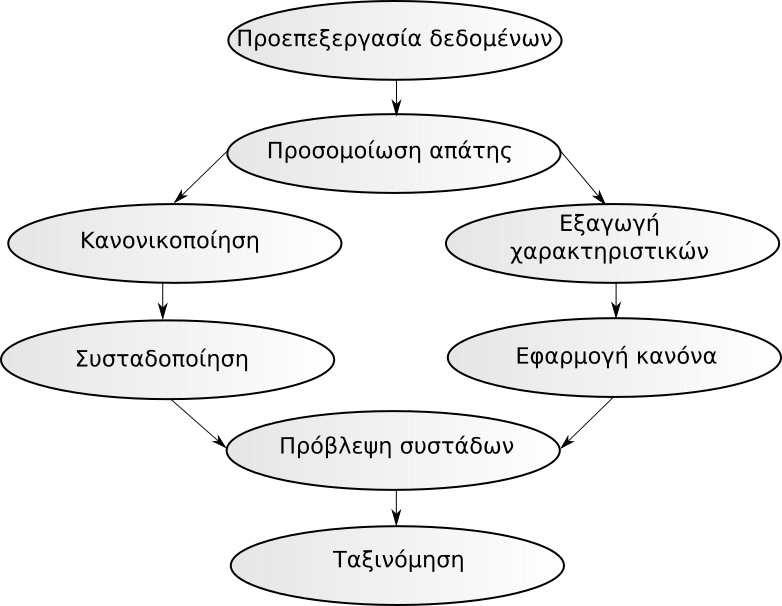
\includegraphics[width=90mm, height=60mm]{../../plots/systems/un_supervised.png}
 \caption{Δομή μη-επιβλεπόμενου ταξινομητή}
\label{fig:unsupervisedsystem}
 \end{figure}
 
\subsection{Μεθοδολογία εξαγωγής αποτελεσμάτων}
Η εξαγωγή αποτελεσμάτων παίζει μεγάλο ρόλο στην τελική απόδοση του αλγορίθμου, οπότε χρειάζεται ιδιαίτερη προσοχή η τοποθέτηση δυαδικών χαρακτηριστικών. Η γενικότερη μεθοδολογία βασίζεται σε δύο σημαντικούς άξονες, καθώς η τομή των δύο είναι αυτή που εξάγει τα βέλτιστα αποτελέσματα. Αυτό γίνεται ξεκάθαρο παρατηρώντας τον πίνακα αποτελεσμάτων \ref{tab:testrules}.\par
Ο πρώτος άξονας αποτελείται από την κανονικοποίηση και την συσταδοποίηση. Κατά την διαδικασία της κανονικοποιήση o πίνακας με τις χρονοσειρές αναστρέφεται, κανονικοποιείται και αναστρέφεται για δεύτερη φορά για να αποκτήσει την ίδια μορφή με την αρχική, αλλά με εύρος τιμών [-1,1]. Με αυτό τον τρόπο δίνεται έμφαση στη μορφή και όχι στα μεγέθη των χρονοσειρών. Έτσι, εκμεταλλεύεται το γεγονός ότι οι χρονοσειρές είναι αρκετά ομοιόμορφες ως προς το σχήμα. Σε επόμενη φάση εκτελείται συσταδοποίηση στα κανονικοποιημένα μεγέθη και διαχωρίζονται οι καταναλωτές σε μια μεγάλη συστάδα με αναμενόμενες μορφές και σε μια μικρή συστάδα με ακανόνιστες συμπεριφορές.\par
Ο δεύτερος άξονας αποτελείται από την εξαγωγή χαρακτηριστικών των χρονοσειρών και την εφαρμοφή του κανόνα. Η εξαγωγή χαρακτηριστικών δίνει τη δυνατότητα μέσω των χαρακτηριστικών διαχωρισμού να δημιουργηθούν ομάδες καταναλωτών που έχουν ύποπτες και αναμενόμενες μετρήσεις. Αν έχουμε έλλειψη χαρακτηριστικών, δηλαδή $0$, πρακτικά σημαίνει πως ο καταναλωτής έχει αναμενόμενη συμπεριφορά. Στην αντίθετη περίπτωση ο καταναλωτής έχει αποκλίνουσα συμπεριφορά και θεωρείται ύποπτος. Εκεί έρχεται ο κανόνας που ορίζει πως αν ο καταναλωτής έχει λιγότερες από τρεις μετρήσεις στα χαρακτηριστικά διαχωρισμού ορίζεται αναμενόμενη συμπεριφορά.
\begin{center}
\begin{longtabu} to 0.8\textwidth { | X[c] || X[c] | X[c] | X[c] | X[c] | X[c] |  }
 \hline
 Κανόνας& \en{DR}  & \en{FPR} & \en{Accuracy} & \en{F1 score} & \en{BDR}\\
\hline
 Συσταδ. & 98.67	&	34.2 &	69.09 &	38.96 &	0.24\\
\hline
 Χαρακτ.& 87.78	&	6.72 &	92.73 &	70.73 &	0.59\\ 
 \hline
 Συνδ. & 89.33	&	5.93 &	93.6 &	73.63 &	0.63\\
\hline
\caption{Δοκιμή στους κανόνες}
\label{tab:testrules}
\end{longtabu}
\end{center}

\section{Δοκιμή αλγορίθμου μη επιβλεπόμενης μάθησης}
Για να επιβεβαιωθεί η ορθή και βέλτιστη λειτουργία του συστήματος απαιτείται δοκιμή των παραμέτρων που το απαρτίζουν. Για να συμβεί αυτό επιλέχθηκαν 4.500 καταναλωτές και αλλοιώθηκαν τα δεδομένα μόνο του 10\%. Ο τύπος απάτης που χρησιμοποιήθηκε για την αλλοίωση των δεδομένων είναι ο πρώτος, καθώς φάνηκε πως είναι ιδιαίτερα πολύπλοκο ακόμη και για επιβλεπόμενο σύστημα να παράξει αξιόπιστα αποτελέσματα.

\subsection{Αποτελέσματα δοκιμής αλγορίθμου}
Παραρώντας την Σχήμα \ref{fig:unsupDRintensity} μπορούμε να παρατηρήσουμε πως έχουμε ομαλή αύξηση του \en{DR} μετά το 0.5, ενώ αντίστοιχα έχουμε ομαλή μείωση του \en{FPR} μετά το ίδιο σημείο. Πριν από το σημείο αυτό οι κυματομορφές έχουν σχετική ασυνέπεια στα αποτελέσματα κάνοντας βίαιες αλλαγές στις μετρικές τους. Πιο συγκεκριμένα στο εύρος [0.4, 0.5] εμφανίζονται δύο μεγάλα πλήγματα στην επίδοση του συστήματος που προδίδουν πως υπό κάποιες συνθήκες το σύστημα δυσκολεύεται να ορίσει την κλοπή, χωρίς όμως να ενοχοποιεί αδίκως.\par

\begin{figure}
\centering
\begin{subfigure}[b]{0.4\textwidth}
 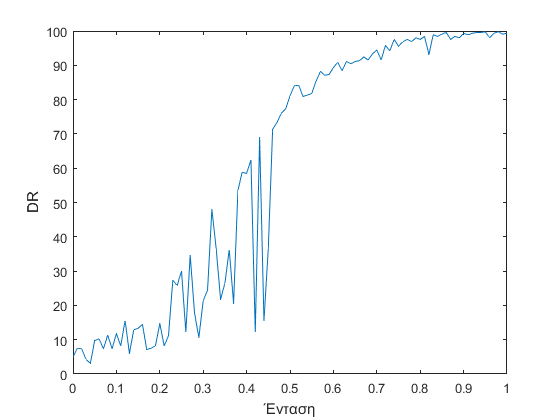
\includegraphics[width=70mm, height=50mm]{../../plots/gr_bigres_dr_intensity_un_sup.png}
\caption{\en{DR} συναρτήσει της έντασης της κλοπής}
\label{fig:unsupDRintensity}
\end{subfigure}
\quad
\begin{subfigure}[b]{0.4\textwidth}
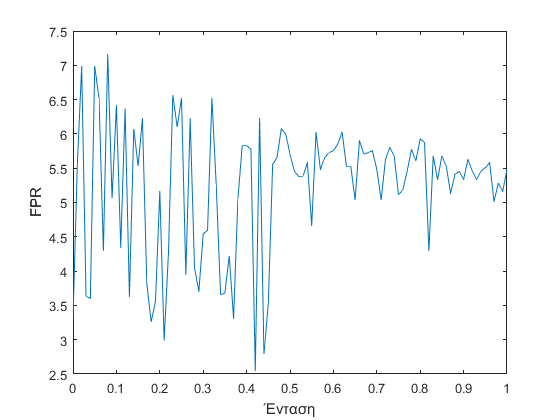
\includegraphics[width=70mm, height=50mm]{../../plots/gr_bigres_fpr_intensity_un_sup.png}
\caption{\en{FPR} συναρτήσει της έντασης της κλοπής}
\label{fig:linearFPRintensity}
\end{subfigure}
\caption{Επίπτωση της έντασης στα αποτελέσματα}
\label{fig:unsupintensityres}
\end{figure}

Παράλληλα, αξίζει να σημειωθεί εδώ πως οι αλγόριθμοι συσταδοποίησης μπορούν να αλλάξουν σε κάποιο βαθμό τα χαρακτηριστικά του συστήματος και την επίδοσή του. Σαν αποτέλεσμα δημιουργήθηκε δοκιμή για τους διαφορετικούς αλγορίθμους που χρησιμοποιήθηκαν στην εξαγωγή των χαρακτηριστικών, καταλήγοντας σε αποτελέσματα για κάθε περίπτωση.
\begin{center}
\begin{longtabu} to 0.8\textwidth { | X[c] || X[c] | X[c] | X[c] | X[c] | X[c] |  }
 \hline
 Αλγ.& \en{DR}  & \en{FPR} & \en{Accuracy} & \en{F1 score} & \en{BDR}\\
\hline
 \en{K-Means} & 86.44	&	5.43 &	93.76 &	73.47 &	0.64\\
\hline
 \en{SOM}& 89.11	&	5.23 &	94.2 &	75.45 &	0.65\\ 
 \hline
  \en{Fuzzy} & 85.78	&	4.99 &	94.09 &	74.37 &	0.66\\
\hline
\caption{Εξερεύνηση συσταδοποιήσεων χαρακτηριστικών στο μη-επιβλεπόμενο σύστημα}
\label{tab:testclusterunsup}
\end{longtabu}
\end{center}
Γίνεται, λοιπόν αντιληπτό πως οι αλγόριθμοι συσταδοποίησης στην εξαγωγή δεδομένων παίζουν σχετικά μικρό ρόλο, αφού τα αποτελέσματα έχουν πολύ μικρές αποκλίσεις μεταξύ τους. Αυτό ήταν κάτι αναμενόμενο βέβαια καθώς μόνο δύο από τα οκτώ χαρακτηριστικά έχουν άμεση συσχέτιση με τη συσταδοποίηση.\par
\subsection{Εξερεύνηση δυνατοτήτων \en{FCM}}
Ο αλγόριθμος ασαφών κ μέσων μέσα από τον παράγοντα ασάφιας δίνει τη δυνατότητα να εξερευνηθούν οι συστάδες και με διαφορετικούς τρόπους. Ειδικότερα, ο παράγοντας αυτός καθορίζει την επικάλυψη των συστάδων. Παράλληλα, για να μπορέσει να διευκρινιστεί τελικά που ανήκει κάθε παράδειγμα παρέχεται μια τιμή για κάθε συστάδα με τη μεγαλύτερη από αυτή να υποδηλώνει μεγάλο βαθμό ομοιότητας του παραδείγματος με τη συστάδα.\par
Με αυτό το σκεπτικό δημιουργήθηκε μια δοκιμή κατά την οποία χωρίς εξαγωγή χαρακτηριστικών ταξινομούνται οι καταναλωτές. Ειδικότερα, γνωρίζοντας το ποσοστό των απατών τίθεται ένα όριο στο πλήθος που επιθυμεί κάποιος να ελέγξει. Ο αλγόριθμος βάση αυτού του πλήθους επιλέγει το δείγμα των καταναλωτών που φαίνεται πιο σίγουρο ότι ανήκει στη συστάδα με ακανόνιστες μετρήσεις. Στην πράξη αν από 450 κλοπές, τεθεί ένα όριο στην εύρεση μόνο των 100, ο αλγόριθμός έχει τη δυνατότητα να αναγνωρίσει σωστά 81, ενώ λάθος 19 όπως φαίνεται και στο παρακάτω σχήμα.\par
\begin{figure}
\centering
 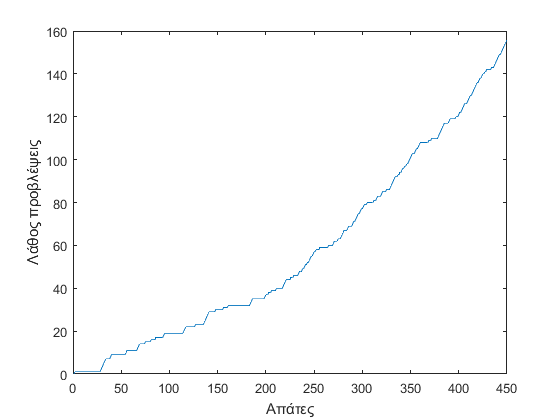
\includegraphics[width=70mm, height=50mm]{../../plots/confident_predictions.png}
\caption{Καμπύλη λάθος προβλέψεων με \en{FCM}}
\label{fig:wrongpredFCM}
\end{figure}
\section{Συστατικά αλγορίθμου ημι-επιβλεπόμενης μάθησης}
Η ημι-επιβλεπόμενη προσέγγιση του προβλήματος επιτυγχάνεται εισάγοντας στο σύστημα μη-επιβλεπόμενης μάθησης νέους αλγορίθμους. Με αυτό τον τρόπο αποκτάται η δυνατότητα εκπαίδευσης με ένα μικρό δείγμα καταναλωτών και των δύο τάξεων ή με μεγαλύτερο δείγμα καταναλωτών της αρνητικής τάξης. Έτσι καλύπτονται και οι δύο δημοφιλέστερες προσεγγίσεις της ημι-επιβλεπόμενης μάθησης. Εν συνεχεία βάση του μοντέλου της εκπαίδευσης ταξινομούνται οι καταναλωτές. Παράλληλα, η προσθήκη νέων αλγορίθμων δίνει τη δυνατότητα εποπτείας των χαρακτηριστικών, αλλά και του μοντέλου που δημιουργήθηκε σε δισδιάστατο χώρο. Οπτικοποιούνται λοιπόν οι πληροφορίες και η εσωτερική λειτουργία του αλγορίθμου, ενώ παράλληλα δίνεται παρέχεται η δυνατότητα εκπαίδευσης προτύπων.\par
Αναλυτικότερα η δομή του αλγορίθμου αναπαρίσταται στο Σχήμα \ref{fig:semisupervisedsystem} ενώ αξίζει να γίνει μια εισαγωγή στα κομμάτια που απαρτίζουν το σύστημα:
\begin{itemize}
\item \em{Προεπεξεργασία δεδομένων}: Επιλέγονται και οργανώνονται τα δεδομένα σε συγκεκριμένους πίνακες και διανύσματα.
\item \em{Προσομοίωση απάτης}: Αλλοιώνονται οι μετρήσεις κάποιων καταναλωτών και ενημερώνονται οι προϋπάρχοντες πίνακες και διανύσματα.
\item \em{Κανονικοποίηση}: Κανονικοποιούνται οι ετήσιες χρονοσειρές και τα χαρακτηριστικά κάθε καταναλωτή σε εύρος τιμών [-1,1] και [0,1] αντίστοιχα.
\item \em{Συσταδοποίηση}: Συσταδοποιούνται οι καταναλωτές με βάση τις κανονικοποιημένες τιμές σε δύο συστάδες. Η μια συστάδα ομαλή και η άλλη η ανώμαλη. 
\item \em{Εξαγωγή χαρακτηριστικών}: Βάση των χρονοσειρών δημιουργούνται ετήσια χαρακτηριστικά για κάθε καταναλωτή, προσπαθώντας να ανιχνευθεί ύποπτη συμπεριφορά.
\item \em{Εφαρμογή κανόνα}: Λαμβάνοντας υπόψη το πλήθος των χαρακτηριστικών απενοχοποίουνται κάποιοι καταναλωτές που βρίσκονται στην ανώμαλη συστάδα.
\item \em{Πρόβλεψη συστάδων}: Θέτονται δυαδικά χαρακτηριστικά στις συστάδες με σεβασμό στον κανόνα.
\item \em{Μείωση διάστασης}: Ο πολυδιάστατος χώρος των χαρακτηριστικών μειώνεται σε δισδιάστατο.
\item \em{Ανίχνευση ανωμαλιών}: Εκπαιδεύεται το μοντέλο πρόβλεψης βάση των χαρακτηριστικών και βελτιστοποιούνται τα όρια ταξινόμησης.
\item \em{Λογικές πράξεις}: Εκτελούνται λογικές πράξεις μεταξύ των δυαδικών χαρακτηριστικών που προέρχονται από την πρόβλεψη συστάδων και την ανίχνευση ανωμαλιών.
\item \em{Ταξινόμηση}: Ταξινομούνται οι καταναλωτές και παράγονται τα τελικά αποτελέσματα και μετρικές.
\end{itemize}

\begin{figure}
\centering
 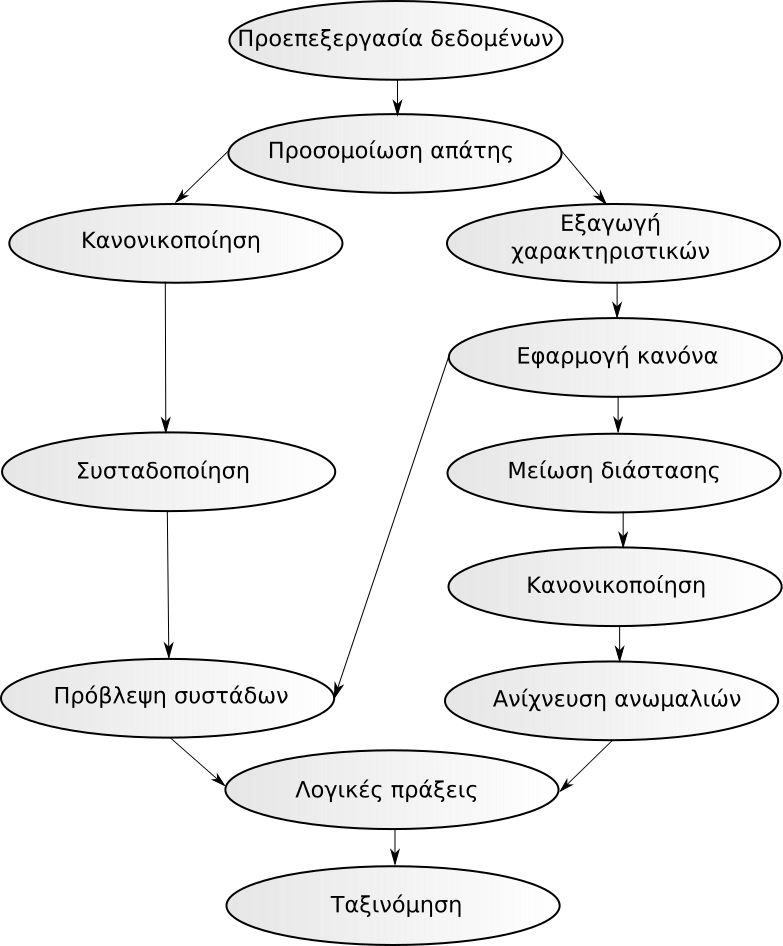
\includegraphics[width=90mm, height=100mm]{../../plots/systems/semi_supervised.png}
 \caption{Δομή ημί-επιβλεπόμενου ταξινομητή}
\label{fig:semisupervisedsystem}
 \end{figure}

\subsection{Εφαρμογή αλγορίθμου μείωσης διάστασης}
Το \en{PCA} είναι ένας μη-επιβλεπόμενος αλγόριθμος γραμμικής μείωσης διάστασης που στοχεύει στην εύρεση μιας βάσης ή ενός συστήματος συντεταγμένων με περισσότερο νόημα για τα δεδομένα και λειτουργεί βάση του πίνακα συνδιακύμανσης για την εύρεση ισχυρών χαρακτηριστικών.\par
Χρησιμοποιείται όταν χρειάζεται να αντιμετωπιστούν οι δυσκολίες των διαστάσεων σε δεδομένα με γραμμικές σχέσεις, καθώς το μεγάλο νούμερο διαστάσεων (χαρακτηριστικών) μπορεί να δημιουργήσει θόρυβο. Το φαινόμενο αυτό επιδεινώνεται όταν τα χαρακτηριστικά έχουν διαφορετικές κλίμακες.\par
Αυτό επιτυγχάνεται μειώνοντας διάσταση δηλαδή χαρακτηριστικά. Αλλά πότε πρέπει να μειώσουμε ή να αλλάξουμε διάσταση?
\begin{itemize}
\item \emph{Καλύτερη εποπτεία και μικρότερη πολυπλοκότητα} Όταν απαιτείται μια πιο ρεαλιστική εποπτεία των διαστάσεων και υπάρχουν πολλά χαρακτηριστικά σε ένα σετ δεδομένων και ειδικότερα όταν υπάρχει διαισθητική γνώση πως δεν απαιτούνται πολλά χαρακτηριστικά.
\item \emph{Καλύτερη οπτικοποίηση}  Όταν είναι αδύνατο να έχουμε καλή οπτικοποίηση λόγω του πλήθους των διαστάσεων χρησιμοποιείται \en{PCA} για να μειωθεί σε μια σκιά με δύο ή τρεις διαστάσεις.
\item \emph{Μείωση μεγέθους} Όταν υπάρχει μεγάλος όγκος δεδομένων και σκοπεύεται να χρησιμοποιηθούν χρονοβόροι αλγόριθμοι στα δεδομένα χρειάζεται να ελαχιστοποιηθούν οι πλεονασμοί.
\item \emph{Διαφορετική οπτική} Όταν υποβόσκει ανάγκη να αυξηθεί η γνώση πάνω στα δεδομένα. Το \en{PCA} μπορεί να δώσει τους καλύτερους γραμμικά ανεξάρτητους και διαφορετικούς συνδιασμούς χαρακτηριστικών, ώστε να περιγραφούν διαφορετικά τα δεδομένα.
\end{itemize}
Η πρακτική υλοποίηση του \en{PCA} είναι εύκολη και συνοψίζεται σε τρία βήματα \cite{PCA}:
\begin{enumerate}
\item Οργάνωση των δεδομένων σε πίνακα $m \times n$, όπου $m$ είναι ο αριθμός των μετρήσεων (χαρακτηριστικών) και $n$ ο αριθμός των δοκιμών.
\item Αφαίρεση του μέσου όρου από κάθε μέτρηση ή από κάθε σειρά.
\item Υπολογισμός \en{SVD} των ιδιοδιανυσμάτων της συνδιακύμανσης.
\end{enumerate}
Η συνδιακύμανση μεταξύ δύο χαρακτηριστικών υπολογίζεται ως εξή:
\begin{center}
$\sigma_{jk}=\frac{1}{n-1}\sum_{i=1}^N(x_{ij}-\bar{x_j})(x_{ik}-\bar{x_k})$
\end{center}
Η παραπάνω μπορεί να γενικευθεί σε υπολογισμό του πίνακα συνδιακύμανσης με την ακόλουθη εξίσωση πινάκων:
\begin{center}
$\Sigma=\frac{1}{n-1}((X-\bar{x})^T(X-\bar{x}))$\\
όπου $\bar{x}$ είναι το διάνυσμα του μέσου όρου $\bar{x}=\sum_{k=1}^nx_i$
\end{center}
Υπάρχουν τρεις προσεγγίσεις οι οποίες αποδίδουν τα ίδια ιδιοδιανύσματα και ζευγάρια ιδιοτιμών:
\begin{itemize}
\item Ιδιοπαραγοντοποίηση του πίνακα συνδιακύμανσης μετά από κανονικοποίηση δεδομένων.
\item Ιδιοπαραγοντοποίηση του πίνακα συσχέτισης.
\item Ιδιοπαραγοντοποίηση του πίνακα συσχέτισης μετά από κανονικοποίηση δεδομένων.
\end{itemize}
Στην παρούσα εργασία παρόλα αυτά χρησιμοποιείται παραγοντοποίηση ιδιόμορφων ιδιοδιανυσμάτων (\en{SVD}) για τη βελτίωση τη υπολογιστική επίδοση \cite{Plotly}.
\subsection{Εφαρμογή αλγορίθμου ανίχνευσης ανωμαλιών}
Ο αλγόριθμος που χρησιμοποιήθηκε για την ανίχνευση ανωμαλιών είναι βασισμένος στο Γκαουσιανό μοντέλο. Τέτοιες τεχνικές υποθέτουν πως τα δεδομένα δημιουργούνται από μια Γκαουσιανή κατανομή. Οι παράμετροι υπολογίζονται με εκτιμητές μέγιστης πιθανοφάνειας (\en{MLE}). Η απόσταση ενός παραδείγματος από το εκτιμώμενο μέσο είναι το αποτέλεσμα του ποσοστού ανωμαλίας. Ορίζεται ένα όριο στα ποσοστά αυτά για να οριστούν οι ανωμαλίες \cite{Anomaly}.\par
Ερμηνεύοντας αυτή την τεχνική πιο φορμαλιστικά θεωρούνται χαρακτηριστικά $x_i$ που υποδεικνύουν ανώμαλα παραδείγματα. Για $m$ παραδείγματα εκπαίδευσης και $n$ χαρακτηριστικά ορίζονται τα δεδομένα εξόδου $\{x^{(1)}, ...,x^{(m)}\}$ που δημιουργούν τη μέση τιμή και διακύμανση κάθε χαρακτηριστικού $\mu_1, ...,\mu_n$,$\sigma_1^2, ..., \sigma_n^2 $.
\begin{center}
$\mu_j=\frac{1}{m}\sum_{i=1}^m x_j^{(i)}$\\ $\sigma_j^2=\frac{1}{m}\sum_{i=1}^m (x_j^{(i)} -\mu_j)^2$\\
\end{center}
Δεδομένου ενός νέου παραδείγματος $x$, υπολογίζεται $p(x)$:\\
\begin{center}
$p(x)=\prod_{j=1}^n p(x_j;\mu_j, \sigma_j^2)=\prod_{j=1}^n \frac{1}{\sqrt{2\pi}\sigma_j}exp(-\frac{(x_j^{(i)} -\mu_j)^2}{2\sigma_j^2})$
\end{center}
Η ανωμαλία λοιπόν ορίζεται αν $p(x)<\epsilon$
Αντίστοιχα το $\epsilon$ είναι προϊόν της διαδικασία βελτιστοποίησης του αλγορίθμου.
\subsection{Μεθοδολογία εξαγωγής αποτελεσμάτων}
Η μεθοδολογία που χρησιμοποιήθηκε σε αυτό το σύστημα κάποια κοινά στοιχεία με τη μεθοδολογία του αλγορίθμου μη-επιβλεπόμενης μάθησης. Συνεπώς, τα αποτελέσματα προέρχονται από δύο βασικές συνιστώσες με την πρώτη να είναι η κανονικοποίηση των καταναλωτών ανά έτος και εν συνεχεία η συσταδοποίησή τους σε δύο συστάδες. Η μία συστάδα έχει αναμενόμενες καταναλωτικές συνήθειες και η άλλη αποτελείται από ασυνήθιστες. H συστάδα με τις ασυνήθιστες συνήθειες βελτιστοποιείται με την παρατήρηση των χαρακτηριστικών διαχωρισμού και έτσι δημιουργείται η πρώτη πρόβλεψη του αλγορίθμου.\par
Παράλληλα, επεκτείνεται η δεύτερη συνιστώσα, για να αποκτηθεί και δεύτερη πρόβλεψη μέσω των χαρακτηριστικών. Ειδικότερα, τα χαρακτηριστικά περνούν από αλγόριθμο μείωσης διάστασης για να γίνει εφικτή η εποπτεία των χαρακτηριστικών σε δισδιάστατο περιβάλλον. Εν συνεχεία χρησιμοποιείται ο αλγόριθμος ανίχνευσης ανωμαλιών για την ολοκλήρωση της δεύτερης πρόβλεψης με δύο διαφορετικές μεθόδους:
\begin{itemize}
\item Η πρώτη μέθοδος εξάγει το μέσο όρο και την διακύμανση από τα μικτά δεδομένα εκπαίδευσης που χρησιμοποιούνται για την εύρεση της πυκνότητας της πολυμεταβλητής κανονικής κατανομής. Τα δεδομένα δοκιμής και τα δυαδικά χαρακτηριστικά τους χρησιμοποιούνται για τη βελτιστοποίηση του ορίου ταξινόμησης για να χρησιμοποιηθεί από τα δεδομένα εκπαίδευσης.
\item Η δεύτερη μέθοδος εκμεταλλεύεται τη γνώση που παράχθηκε από την πρώτη συνιστώσα εκπαιδεύοντας το μοντέλο μόνο με αρνητικά παραδείγματα που χρησιμοποιούνται για την εύρεση της πυκνότητας της πολυμεταβλητής κανονικής κατανομής στο ένα κομμάτι των δεδομένων δοκιμής. Το άλλο κομμάτι των δεδομένων δοκιμής και τα δυαδικά χαρακτηριστικά τους χρησιμοποιούνται για τη βελτιστοποίηση του ορίου ταξινόμησης που εφαρμόζεται στο πρώτο κομμάτι δεδομένων δοκιμής.
\end{itemize}
\par Και οι δύο μέθοδοι εξάγουν δυαδικές προβλέψεις για τη δεύτερη συνιστώσα, ολοκληρώνοντας με αυτό τον τρόπο τις προβλέψεις του ταξινομητή. Δεδομένου ότι ο ταξινομητής πρέπει να έχει μια και μόνο εκτίμηση τα δύο δυαδικά χαρακτηριστικά εκτελούν μεταξύ τους απλές δυαδικές πράξεις που καταλήγοντας στην τελική πρόβλεψη του αλγορίθμου.
\section{Δοκιμή αλγορίθμων ημι-επιβλεπόμενης μάθησης}
Σκοπός των αλγορίθμων ημι-επιβλεπόμενης μάθησης είναι να παραχθούν βελτιωμένα αποτελέσματα που να προσεγγίζουν τα αποτελέσματα της επιβλεπόμενης μάθησης. Αυτό δεν είναι εύκολα εφικτό παρόλα αυτά, καθώς οι συγκεκριμένοι αλγόριθμοι χρησιμοποιούν μόνο το 30\% των δυαδικών χαρακτηριστικών, ενώ οι επιβλεπόμενοι αλγόριθμοι το 70\%.\par
Έτσι, και εδώ όπως και στις άλλες δοκιμές χρησιμοποιήθηκαν 4.500 καταναλωτές με 10\% να έχουν αλλοιωμένες μετρήσεις.  Η κανονικοποίηση των ετήσιων χρονοσειρών επιτεύχθηκε σε εύρος [-1,1], ενώ η κανονικοποίηση των χαρακτηριστικών σε εύρος [0,1].
\subsection{Εξερεύνηση λογικών πράξεων στους ημι-επιβλεπόμενους αλγόριθμους}
Αρχικά αξίζει να παρατηρηθεί ποια λογική πράξη στην εξαγωγή αποτελεσμάτων παρουσιάζει τα βέλτιστα αποτελέσματα. Η χρήση της \en{OR} αναμένεται να διευρύνει τα όρια του ταξινομητή, αλλά αν η δεύτερη συνιστώσα του ταξινομητή είναι εξαιρετικά εύστοχη οι λάθος προβλέψεις δεν θα αυξηθούν σε μεγάλο βαθμό. Από την άλλη η χρήση της \en{AND} αναμένεται να μειώσει τις λάθος προβλέψεις και να κάνει τον αλγόριθμο πιο προσεκτικό στην επιλογή της απάτης. Στον πίνακα παρακάτω οι παραπάνω υποθέσεις παίρνουν σάρκα και οστά.
\begin{center}
\begin{longtabu} to 0.8\textwidth { | X[c] || X[c] | X[c] | X[c] | X[c] | X[c] |  }
 \hline
 Πύλη & \en{DR}  & \en{FPR} & \en{Accuracy} & \en{F1 score} & \en{BDR}\\
\hline
 \en{AND} & 72.01 & 2.68 & 94.76 & 73.52 & 0.75\\
 \hline
 \en{OR}& 91.08 & 7.61 &  92.25 & 70.81 & 0.57\\ 
\hline
\caption{Εξερεύνηση λογικών πράξεων στο τυπικό ημι-επιβλεπόμενο σύστημα}
\label{tab:testlogicopersemisup1}
\end{longtabu}
\end{center}

\begin{center}
\begin{longtabu} to 0.8\textwidth { | X[c] || X[c] | X[c] | X[c] | X[c] | X[c] |  }
 \hline
 Πύλη & \en{DR}  & \en{FPR} & \en{Accuracy} & \en{F1 score} & \en{BDR}\\
\hline
 \en{AND} & 90.63 & 10.58 & 89.65 & 77.33 & 0.49\\
 \hline
 \en{OR}& 98.11 & 28.59 & 76.38 & 60.73 & 0.28\\ 
\hline
\caption{Εξερεύνηση λογικών πράξεων στο εναλλακτικό ημι-επιβλεπόμενο σύστημα}
\label{tab:testlogicopersemisup2}
\end{longtabu}
\end{center}

\subsection{Εξερεύνηση συσταδοποιήσεων στους ημι-επιβλεπόμενους αλγόριθμους}
Βάση των αποτελεσμάτων του \en{F1 score} και του \en{Accuracy} επιλέγεται η πύλη \en{AND}, καθώς δεν δίνεται μεγαλύτερη βάση στην γενική απόδοση του αλγορίθμου από την απόλυτη ακρίβεια στον εντοπισμό των μη τεχνικών απωλειών. Ειδικότερα το υψηλότερο \en{F1 score} προδίδει πως υποβόσκει πολύ μικρό ποσοστό στη λάθος πρόβλεψη και ικανοποιητικό ποσοστό στον εντοπισμό της.\par
Στη συνέχεια επιλέγεται να γίνει αναλυτική δοκιμή των συσταδοποιήσεων των χρονοσειρών και των χαρακτηριστικών. Δυστυχώς η συσταδοποίηση \en{SOM} αδυνατεί να ολοκληρώσει συσταδοποίηση στις χρονοσειρές. Παρόλα, αυτά έγινε διεξοδική εξερεύνηση των συσταδοποιήσεων. Από προηγούμενα αποτελέσματα αναμένεται να μην παρατηρηθούν μεγάλες αποκλίσεις στα αποτελέσματα.
\begin{center}
\begin{longtabu} to 0.8\textwidth { | X[c] || X[c] | X[c] | X[c] | X[c] | X[c] |  }
 \hline
 Αλγ.& \en{DR}  & \en{FPR} & \en{Accuracy} & \en{F1 score} & \en{BDR}\\
\hline
 \en{K-Means} & 71.09 & 2.00 & 95.49 & 74.64 & 0.80\\
 \hline
 \en{K-M-SOM}& 76.85 & 3.06 & 94.95 & 75.04 & 0.74\\ 
\hline
 \en{FCM-SOM}& 79.48& 3.83 & 94.54 & 73.94 & 0.70\\ 
 \hline
  \en{Fuzzy} & 78.77 & 3.75 & 94.44 & 74.53 & 0.70\\
\hline
\caption{Εξερεύνηση συσταδοποιήσεων στο τυπικό ημι-επιβλεπόμενο σύστημα}
\label{tab:testclustersemisup1}
\end{longtabu}
\end{center}

\begin{center}
\begin{longtabu} to 0.8\textwidth { | X[c] || X[c] | X[c] | X[c] | X[c] | X[c] |  }
 \hline
 Αλγ.& \en{DR}  & \en{FPR} & \en{Accuracy} & \en{F1 score} & \en{BDR}\\
\hline
 \en{K-Means} & 91.15 & 10.96  & 89.45 & 77.01 & 0.48\\
 \hline
 \en{K-M-SOM}& 91.89 & 10.21  & 90.21 & 78.92 & 0.50\\ 
\hline
 \en{FCM-SOM}& 91.90 & 9.04  & 91.13 & 79.37 & 0.53\\ 
 \hline
  \en{Fuzzy} & 89.32 & 9.23  & 90.51 & 76.98 & 0.52\\
\hline
\caption{Εξερεύνηση συσταδοποιήσεων στο εναλλακτικό ημι-επιβλεπόμενο σύστημα}
\label{tab:testclustersemisup2}
\end{longtabu}
\end{center}
\subsection{Εξερεύνηση μείωσης διάστασης στους ημι-επιβλεπόμενους αλγόριθμους}
Σε αυτό το σημείο αξίζει να παρατηρήσουμε τους ορίζοντες που ανοίγει ο αλγόριθμος μείωσης διάστασης. Αρχικά δίνει τη δυνατότητα να έχουμε εποπτεία σε όλο το σετ δεδομένων και επίσης να παρατηρήσουμε τα όρια που θέτει ο αλγόριθμος ανίχνευσης ανωμαλιών.\par
Στο Σχήμα \ref{fig:charclasscons} παρατηρείται η αποτύπωση που δημιουργεί η μείωση διάστασης στα χαρακτηριστικά των καταναλωτών. Τα κυκλικά κίτρινα σημεία είναι η αρνητική ομάδα, ενώ οι μαύροι σταυροί είναι η θετική ομάδα. Από την κατανομή της αρνητική τάξη εύκολα γίνεται αντιληπτό οι περισσότεροι καταναλωτές βρίσκονταί κοντά στο κέντρο των αξόνων. Αντίστοιχα η θετική τάξη αποτυπώνεται κάτων από το κέντρο των αξόνων μαζί με λίγα αρνητικά παραδείγματα. Γίνεται συνεπώς αντιληπτό πως τα σύνολα δεν είναι πλήρως διαχωρίσιμα και για αυτό το λόγο αναμένεται τα αποτελέσματα με μείωση διάστασης να είναι χειρότερα. Η δυσκολία αυτή παρόλα αυτά παρακάμπτεται με την πρώτη συνιστώσα της ταξινόμησης.\par
\begin{figure}
 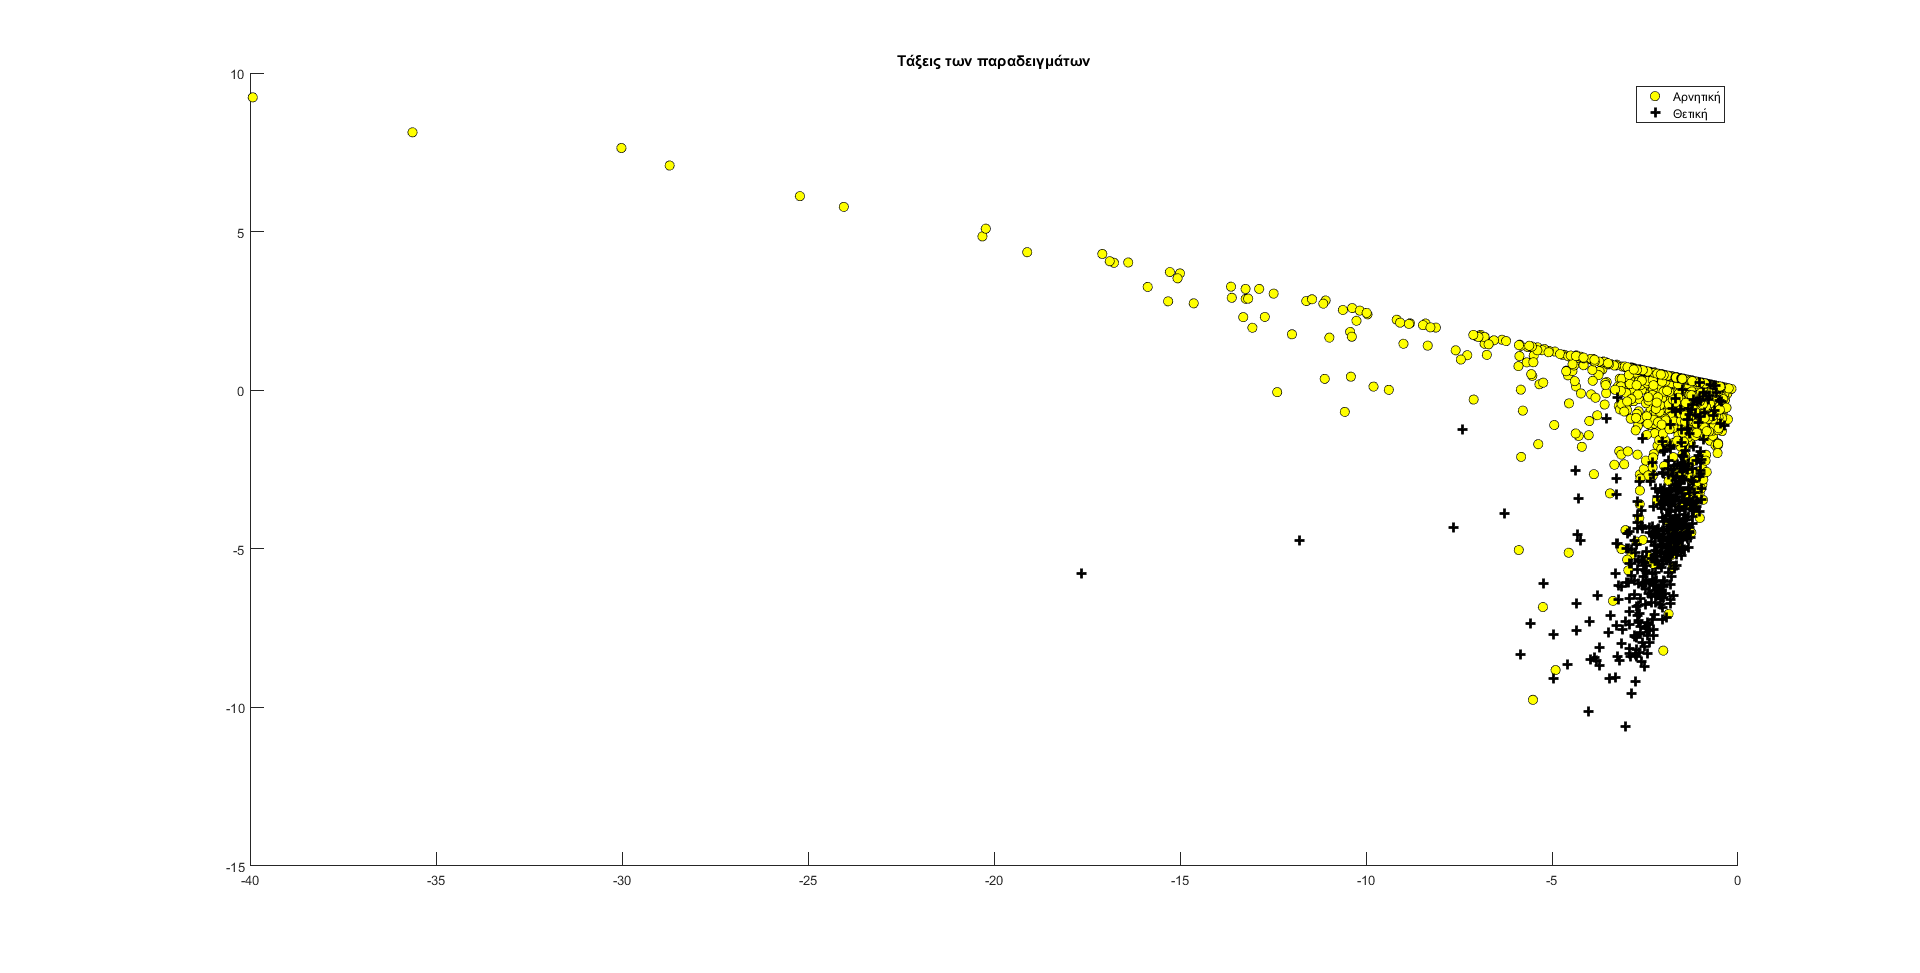
\includegraphics[width=160mm, height=100mm]{../../plots/gr_class_semi_sup.png}
\caption{Χαρακτηριστικά και τάξεις καταναλωτών}
\label{fig:charclasscons}
\end{figure}
Στο Σχήμα \ref{fig:viewandthreshold} παρατηρείται η οριοθέτηση που θέτει ο αλγόριθμος ανίχνευσης ανωμαλειών. Στην πρώτη περίπτωση είναι εμφανές πως η κίτρινη γραμμή κάνει ένα σαφή διαχωρισμό στις δύο κλάσεις ενώ στη δεύτερη περίπτωση η οριοθέτηση δεν είναι τόσο σαφής και περιλαμβάνει μεγάλο κομμάτι όλων των δεδομένων. Με το παραπάνω υπόψη γίνεται για άλλη μια φορά σαφές πως η μείωση διαστάσεων δεν βοηθά στην βελτιστοποίηση του αλγορίθμου άμεσα, αλλά δίνει μια άλλη οπτική των δεδομένων.
\begin{figure}
\begin{subfigure}[b]{0.4\textwidth}
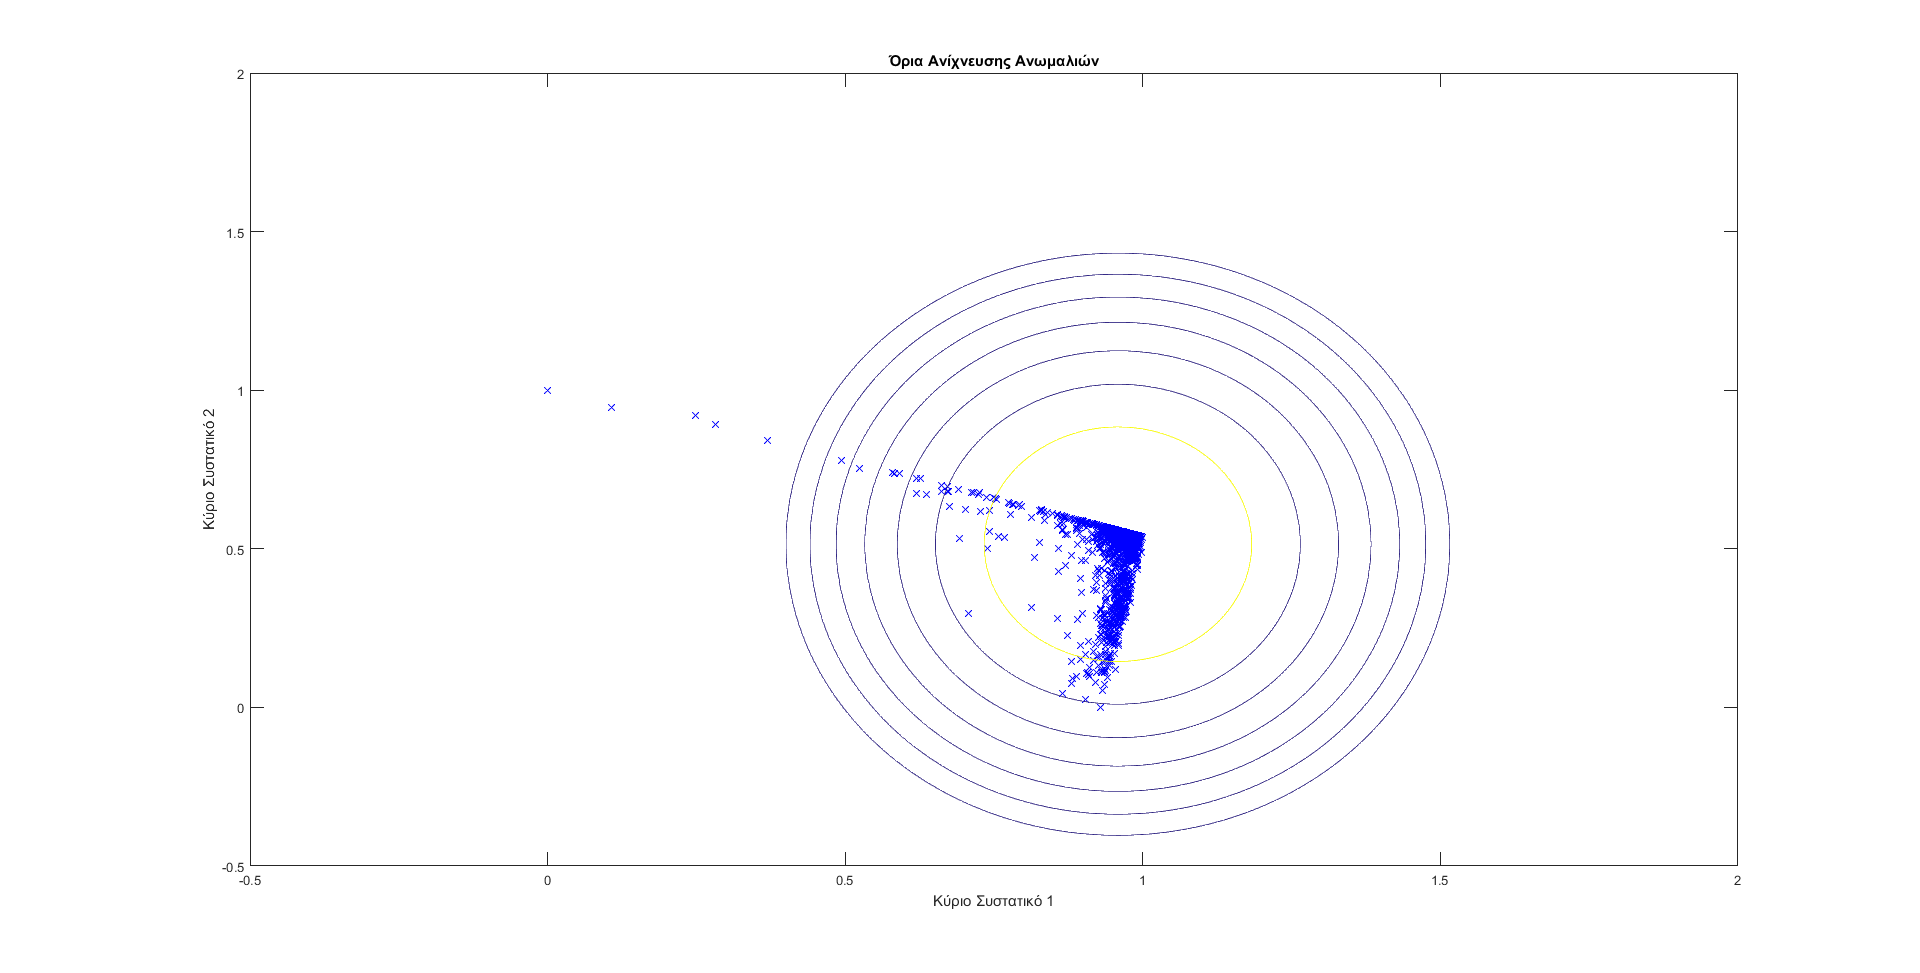
\includegraphics[width=160mm, height=100mm]{../../plots/gr_threshold_semi_sup_1.png}
\caption{Όρια τυπικής ανίχνευσης ανωμαλιών}
\label{fig:threshanomalydetection1}
\end{subfigure}

\begin{subfigure}[b]{0.4\textwidth}
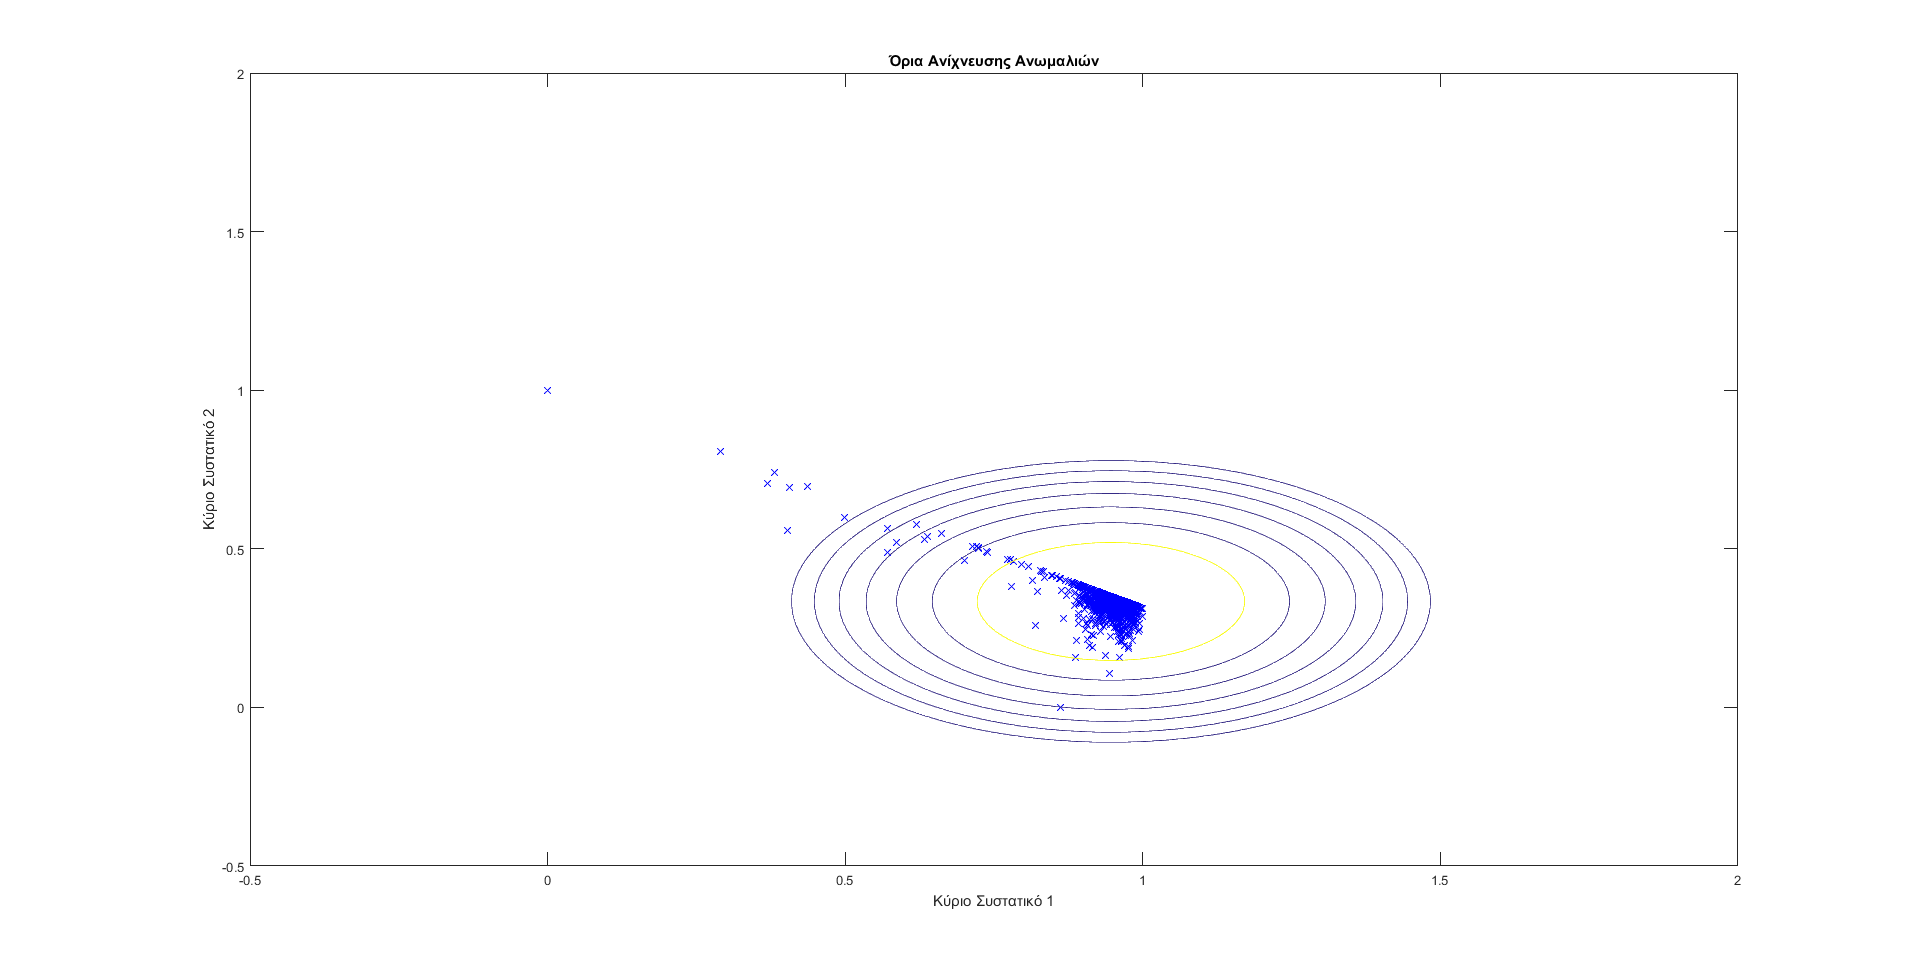
\includegraphics[width=160mm, height=100mm]{../../plots/gr_threshold_semi_sup_2.png}
\caption{Όρια εναλλακτικής ανίχνευσης ανωμαλιών}
\label{fig:threshanomalydetection2}
\end{subfigure}

\caption{Όρια ανίχνευσης ανωμαλιών}
\label{fig:viewandthreshold}
\end{figure}

Για να αποδειχθεί και με αποτελέσματα η παραπάνω υπόθεση γίνεται μια νέα σειρά δοκιμών με τον αλγόριθμο μείωσης διάστασης.
\begin{center}
\begin{longtabu} to 0.8\textwidth { | X[c] || X[c] | X[c] | X[c] | X[c] | X[c] |  }
 \hline
 Αλγ.& \en{DR}  & \en{FPR} & \en{Accuracy} & \en{F1 score} & \en{BDR}\\
\hline
 τυπικός & 79.01 & 2.51 & 95.59 & 78.65 & 0.78\\
 \hline
 εναλλ\en{AND}& 0.00 & 0.00  & 80.28 &  - &  -\\ 
\hline
 εναλλ\en{OR}& 87.85 & 11.79  & 88.14 & 73.44 & 0.45\\ 
 \hline
\caption{Εξερεύνηση μείωσης διάστασης στους ημι-επιβλεπόμενους αλγορίθμους}
\label{tab:testpcasemisup}
\end{longtabu}
\end{center}
\subsection{Αποτελέσματα δοκιμής αλγορίθμου}
Για την τελική δοκιμή επιλέχθηκαν όλοι οι πιθανοί καταναλωτές και εισάχθηκε 10\%. Ένας ικανοποιητικός τρόπος να παρατηρηθεί η λειτουργία του αλγορίθμου είναι να δοκιμαστεί το σύστημα υπό διαφορετικές εντάσεις κλοπής. Έτσι επιλέχθηκαν τα συστήματα με \en{K-Means}, χωρίς μείωση διάστασης και πύλες \en{AND} που είχαν τα πιο συνεπή αποτελέσματα.\par
Στον τυπικό αλγόριθμο παρατηρούνται ομαλές καμπύλες με τα συνεχή αύξουσα πορεία στο \en{DR} και σχεδόν συνεχή φθίνουσα στο \en{FPR}. Παράλληλα, αξίζει να σημειωθεί πως ενώ το \en{DR} δεν φτάνει το 100\% αλλά το 90\%, το \en{FPR} φτάνει σε εξαιρετικά χαμηλά επίπεδα που ουσιαστικά σημαίνει ότι πρόκειται για ένα αρκετά συμπαγή και έμπιστο σύστημα.\par
Από την άλλη πλευρά ο εναλλακτικός αλγόριθμος έχει και αυτός ομαλή καμπύλη \en{DR} με αύξουσα κυρίως πορεία, αλλά η καμπύλη \en{FPR} έχει ιδιαίτερα περίεργη συμπεριφορά. Το σύστημα φαίνεται πως όσο η ένταση αντί να αυξάνει τη σιγουριά του ως προς την απάτη, αυξάνει σε τόσο μεγάλο ποσοστό την ενοχοποίηση που επιλέγει πιο αυθαίρετα την θετική κλάση με αποτέλεσμα την σταδιακή αύξηση και των δύο μετρικών.
\begin{figure}
\centering
\begin{subfigure}[b]{0.4\textwidth}
 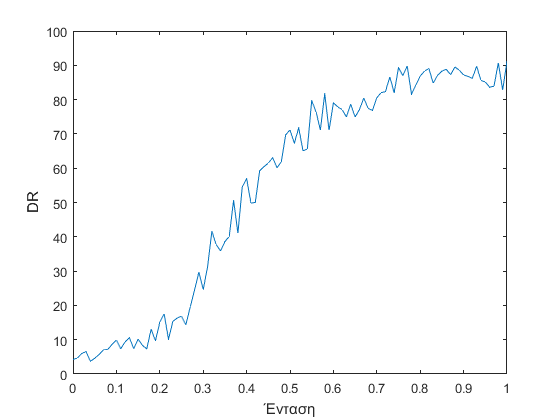
\includegraphics[width=70mm, height=50mm]{../../plots/gr_dr_intensity_semi_sup1.png}
\caption{\en{DR} συναρτήσει της έντασης του τυπικού αλγορίθμου}
\label{fig:testintdrsemisup1}
\end{subfigure}
\quad
\begin{subfigure}[b]{0.4\textwidth}
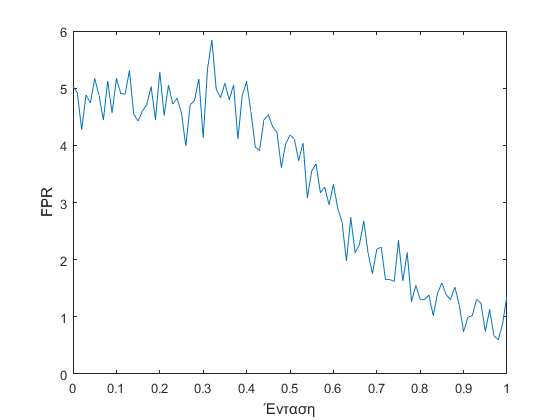
\includegraphics[width=70mm, height=50mm]{../../plots/gr_fpr_intensity_semi_sup1.png}
\caption{\en{FPR} συναρτήσει της έντασης του τυπικού αλγορίθμου}
\label{fig:testintfprsemisup1}
\end{subfigure}
\quad
\begin{subfigure}[b]{0.4\textwidth}
 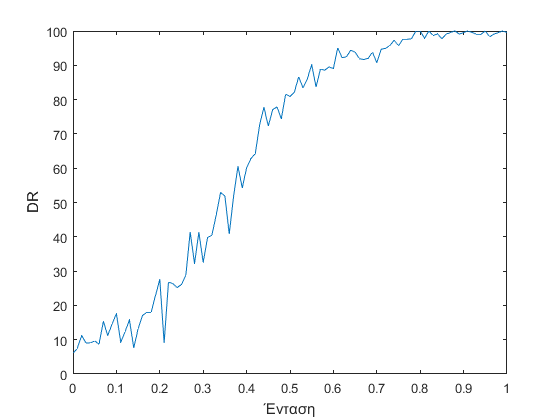
\includegraphics[width=70mm, height=50mm]{../../plots/gr_dr_intensity_semi_sup2.png}
\caption{\en{DR} συναρτήσει της έντασης του εναλλακτικού αλγορίθμου}
\label{fig:testintdrsemisup2}
\end{subfigure}
\quad
\begin{subfigure}[b]{0.4\textwidth}
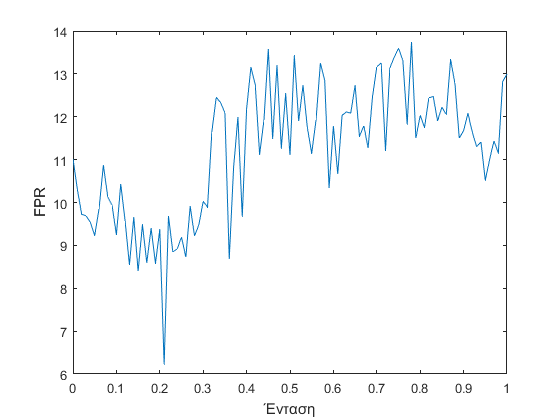
\includegraphics[width=70mm, height=50mm]{../../plots/gr_fpr_intensity_semi_sup2.png}
\caption{\en{FPR} συναρτήσει της έντασης του εναλλακτικού αλγορίθμου}
\label{fig:testintfprsemisup2}
\end{subfigure}

\caption{Δοκιμή έντασης ημι-επιβλεπόμενων συστημάτων}
\label{fig:testintensitysemisup}
\end{figure}

\section{Σχόλια}
Στο παρόν κεφάλαιο έγινε μια διεξοδική αναζήτηση μη-επιβλεπόμενων και ημι-επιβλεπόμενων συστημάτων με σκοπό την άμεση σύγκριση με τον αλγόριθμο επιβλεπόμενης μάθησης. Τα αποτελέσματα δείχνουν πως μπορεί να υπάρξει σύστημα που εντοπίζει μη τεχνικές απώλειες χωρίς καμία εκπαίδευση και χωρίς τη χρήση δυαδικών χαρακτηριστικών. Παράλληλα, η επίδοση του ημι-επιβλεπόμενου συστήματος δίνει τη δυνατότητα κατανόησης πως ακόμη και με λίγα δυαδικά χαρακτηριστικά ο μη-επιβλεπόμενος αλγόριθμος μπορεί να γίνει πιο αξιόπιστος στην αναγνώριση απάτης και να βελτιώσει την επίδοσή του. Συγκρίνοντας τους ημι-επιβλεπόμενους αλγόριθμους γίνεται φανερό πως η τυπική ανίχνευση ανωμαλιών είναι γενικών πιο προβλέψιμη και πιο εύστοχη.\par
Συνοψίζοντας καθίσταται σαφές πως οι δύο συνιστώσες ταξινόμησης είναι απαραίτητες για την εξαγωγή ικανοποιητικών μετρικών και πως η αλληλεπίδρασή τους κάνει την ταξινόμηση αξιόπιστη. Από την άλλη πλευρά,  η μέθοδος συσταδοποίησης δεν έχει εξαιρετική σημασία για την απόδοση του συστήματος ακόμη και όταν αλλάζει η μέθοδος και στους δύο άξονες ταξινόμησης. Τέλος, για την αύξηση εμπιστοσύνης στα συστήματα απαιτείται η χρήση της πύλης \en{AND} για την τελική δυαδική πράξη των ταξινομητών, καθώς επιτυγχάνει ικανοποιητικά αποτελέσματα σε δύο πολύ σημαντικές μετρικές, το \en{F1 score} και το \en{Accuracy}.